\documentclass{egee}
%\usepackage{doxygen}

%
%% Copyright (c) Members of the EGEE Collaboration. 2004-2010.
%% See http://www.eu-egee.org/partners for details on the copyright holders.
%% 
%% Licensed under the Apache License, Version 2.0 (the "License");
%% you may not use this file except in compliance with the License.
%% You may obtain a copy of the License at
%% 
%%     http://www.apache.org/licenses/LICENSE-2.0
%% 
%% Unless required by applicable law or agreed to in writing, software
%% distributed under the License is distributed on an "AS IS" BASIS,
%% WITHOUT WARRANTIES OR CONDITIONS OF ANY KIND, either express or implied.
%% See the License for the specific language governing permissions and
%% limitations under the License.
%
% external packages
\usepackage{xspace}
\usepackage{ifthen}
\usepackage{comment}

% useful definitions
\def\LB{L\&B\xspace}
\def\LBnew{\LB version 2.0\xspace}
\def\LBold{\LB version 1.x\xspace}
\def\JP{JP\xspace}
%\def\eg{e.\,g.}
\def\eg{for example\xspace}
\def\Eg{For example\xspace}
%\def\ie{i.\,e.}
\def\ie{that is\xspace}
\def\wrt{with respect to\xspace}
\def\Dash{---\penalty-1000}

\def\req{\noindent\textbf{Prerequisities:}}
\def\how{\noindent\textbf{How to run:}}
\def\what{\noindent\textbf{What to test:}}
\def\result{\noindent\textbf{Expected result:}}
\def\note{\noindent\textbf{Note:}}
\def\path#1{{\normalfont\textsf{#1}}}
\def\code#1{\texttt{#1}}
\def\ctblb#1{\code{org.glite.testsuites.ctb/LB/tests/#1}}

\specialcomment{hints}{\par\noindent\textbf{Hints: }\begingroup\slshape}{\endgroup}
%\includecomment{hints}

\long\def\TODO#1{\par\noindent\textbf{TODO:} {\sl#1}\par}
\long\def\ludek#1{}

\hyphenation{plug-in}

\newcommand{\email}[1]{\href{mailto:#1}{#1}}

\input{ver.tex}


\title{Logging and Bookkeeping}
\Subtitle{User's Guide}
\author{CESNET EGEE II JRA1 team}
\DocIdentifier{EGEE-II....}
\Date{\today}
\Activity{JRA1: Middleware Engineering and Integration}
\DocStatus{DRAFT}
\Dissemination{PUBLIC}
\DocumentLink{http://...}

\Abstract{
This user's guide explains how to use the Logging and Bookkeeping (\LB) service. 
The service architecture is described briefly. 
Examples on using \LB\ event logging command to log a~user tag and change job ACL are given,
as well as \LB\ query and notification API use cases.
% The reference section contains complete description of both the logging command and the API's.
}

\begin{document}

\begin{center}
{\bf Delivery Slip}
\end{center}
\begin{tabularx}{\textwidth}{|l|l|l|X|X|}
\hline
           & {\bf Name} & {\bf Partner} & {\bf Date} & {\bf Signature} \\
\hline
{\bf From} & Ale\v{s} K\v{r}enek & CESNET & August 1, 2008 & \\
\hline
{\bf Reviewed by} & &  & & \\

\hline
{\bf Approved by} & & & & \\
\hline
\end{tabularx}

\begin{center}
{\bf Document Change Log}
\end{center}

\begin{tabularx}{\textwidth}{|l|l|X|X|}
\hline
{\bf Issue } & {\bf Date  } & {\bf Comment } & {\bf Author  } \\   \hline
1.0.0 & August 1, 2008 & Initial version & CESNET team \\

\hline
\end{tabularx}

\begin{center}
{\bf Document Change Record}
\end{center}

\begin{tabularx}{\textwidth}{|l|l|X|}
\hline
{\bf Issue } & {\bf Item  } & {\bf Reason for Change } \\   \hline

\hline
\end{tabularx}

% Taken from:
% https://twiki.cern.ch/twiki/bin/view/EGEE/EGEEgLiteSoftwareLicense
%
\vfill{}

{\bf
Copyright} \copyright\ {\bf Members of the EGEE Collaboration. 2004.  See
\href{http://www.eu-egee.org/partners/}{http://www.eu-egee.org/partners/} for
details on the copyright holders.  

Licensed under the Apache License, Version 2.0 (the "License"); you may not use
this file except in compliance with the License.  You may obtain a copy of the
License at 

\begin{center}
\href{http://www.apache.org/licenses/LICENSE-2.0}{http://www.apache.org/licenses/LICENSE-2.0}
\end{center}

Unless required by applicable law or agreed to in writing, software distributed
under the License is distributed on an "AS IS" BASIS, WITHOUT WARRANTIES OR
CONDITIONS OF ANY KIND, either express or implied.  See the License for the
specific language governing permissions and limitations under the License.
}


\clearpage

\newpage
\tableofcontents

\newpage
%
%% Copyright (c) Members of the EGEE Collaboration. 2004-2010.
%% See http://www.eu-egee.org/partners for details on the copyright holders.
%% 
%% Licensed under the Apache License, Version 2.0 (the "License");
%% you may not use this file except in compliance with the License.
%% You may obtain a copy of the License at
%% 
%%     http://www.apache.org/licenses/LICENSE-2.0
%% 
%% Unless required by applicable law or agreed to in writing, software
%% distributed under the License is distributed on an "AS IS" BASIS,
%% WITHOUT WARRANTIES OR CONDITIONS OF ANY KIND, either express or implied.
%% See the License for the specific language governing permissions and
%% limitations under the License.
%
%
%% Copyright (c) Members of the EGEE Collaboration. 2004-2010.
%% See http://www.eu-egee.org/partners for details on the copyright holders.
%% 
%% Licensed under the Apache License, Version 2.0 (the "License");
%% you may not use this file except in compliance with the License.
%% You may obtain a copy of the License at
%% 
%%     http://www.apache.org/licenses/LICENSE-2.0
%% 
%% Unless required by applicable law or agreed to in writing, software
%% distributed under the License is distributed on an "AS IS" BASIS,
%% WITHOUT WARRANTIES OR CONDITIONS OF ANY KIND, either express or implied.
%% See the License for the specific language governing permissions and
%% limitations under the License.
%
\section{\LB Architecture}

%historie: vyrobeno pro WMS v EDG, 1. a 2. verze (seq. ��sla,
%cache a dotazy na stavy), v EGEE gLite---ustabiln�n�, proxy

\LB's primary purpose is tracking WMS jobs as they are processed by
individual Grid components, not counting on the WMS to provide this data.
The information gathered from individual sources is collected, stored in
a database and made available at a single contact point. The user gets a
complete view on her job without the need to inspect several service logs
(which she may not be authorized to see in the entirety or she may not be
even aware of their existence).

While \LB keeps track of submitted and running jobs, the information is
kept by the \LB service also after the job has been finished (successfully
completed its execution, failed, or has been canceled for any reason). The 
information is usually available several days after the last event
related to the job arrived, to give user an opportunity to check the job's
final state and eventually evaluate failure reasons.

As \LB collects also information provided by the WMS, the WMS services are
no longer required to provide a job-state querying interface.  Most of the
WMS services can be even designed as stateless---they process a~job and
pass it over to another service, not keeping state information about the job
anymore.  During development and deployment of the first WMS version this
approach turned to be essential in order to scale the services to the
required extent~\cite{jgc}. 

\LB must collect information about all important events in the Grid job
life. These include transitions between components or services, results
of matching and brokerage, waiting in queue systems or start and end of
actual execution.
We decided to achieve this
goal through provision of an API (and the associated library) and
instrumenting individual WMS services and other Grid components with direct
calls to this API. But as \LB is a centralized service (there exists 
a single point where all information about a particular job must
eventually arrive), direct synchronous transfer of data could have
prohibiting impact on the WMS operation.
The temporary unavailability or overload of the remote \LB service
must not prevent (nor block) the instrumented service to perform as usual.
An asynchronous model with a clear \emph{asynchronous delivery
semantics}, see Sect.~\ref{gathering}, is used to address this issue.

As individual Grid components have only local and transient view of a
job, they are able to send only information about individual events. This
raw, fairly complex information is not 
a~suitable form to be presented to the user for frequent queries. It must
be processed at the central service and users must be presented primarily with this
processed form. This form is derived from the \emph{job state} and its
transition, not from the job events themselves. The raw information is
still available, in case more detailed insight is necessary.

While the removal of state information from (some of) the WMS services
helped to achieve the high scalability of the whole WMS, the state
information is still essential for the decisions made within the resource
broker or during the matchmaking process. 
\Eg decision on job resubmission is usually affected by the number of
previous resubmission attempts. This kind of information is currently
available in the \LB only, so the next ``natural'' requirement has been
to provide an interface for WMS (and other) services to the \LB to query
for the state information. However, this requirement contains two
contradictions: (i)~due to the asynchronous event delivery model, the \LB
information may not be up to date and remote queries may lead to unexpected
results
(or even inconsistent ones---some older information may not be available for 
one query but may arrive before a subsequent query is issued),
and (ii)~the dependence on a~remote service to provide vital state information
may block the local service if the remote one is not responding.
These problems are addressed by providing \emph{local view} on the \LB data,
see Sect.~\ref{local}.




\subsection{Concepts}


\subsubsection{Jobs and events}
To keep track of user jobs on the Grid, we first need some reliable
way to identify them. This is accomplished by assigning a unique
identifier, which we call \emph{jobid} (``Grid jobid''), to every job
before it enters the Grid. A~unique jobid is assigned, making it the
primary index to unambiguously identify any Grid job. This jobid is then
passed between Grid
components together with the job description as the job flows through
the Grid; the components themselves may have (and usually do) their
own job  identifiers, which are unique only within these components.

Every Grid component dealing with the job during its lifetime 
may be a source of information about the job. The \LB gathers information
from all the 
relevant components. This information is obtained in the form of
\LB events, pieces of data generated by Grid components, which mark
important points in the job lifetime (\eg passing of job control
between the Grid components are important milestones in job lifetime
independently on the actual Grid architecture); see Appendix~\ref{a:events}
for a~complete list. We collect those
events, store them into a database and simultaneously process them to
provide higher level view on the job's state.  The \LB collects redundant
information---the event scheme has been designed to be as redundant as
possible---and this redundancy is used to improve resiliency in a
presence of component or network failures, which are omnipresent on any
Grid. 

The \LB events themselves are structured into \emph{attribute}~=
\emph{value} pairs, the set of required and optional attributes is defined by the
event \emph{type} (or scheme). For the purpose of tracking job status on
the Grid and with the knowledge of WMS Grid middleware structure we
defined an \LB schema with specific \LB event
types (see Appendix\ref{a:events}).
The schema contains a common base, the attributes that must be assigned
to every single event. The primary key is the jobid, which is also one of
the required attributes. Among other common attributes belong currently the
timestamps of the event origin and of the event arrival to LB, 
generating component name, the event type, its priority and sequence code 
(see Sect.~\ref{evprocess}) and so on. For a complete list of attributes
see \cite{lbdg}.

While the necessary and sufficient condition for a global jobid is
to be Grid-wide unique, additional desired property relates to the
transport of events through the network: All events belonging to the same
job must be sent to the same \LB database. This must be done on a~per
message basis, as each message may be generated by a different component.
The same problem is encountered
by users when they look for information about their job---they need
to know where to find the appropriate \LB database too.
While it is possible to devise a global service where each job registers
its jobid together with the address of the appropriate database, such a
service could easily become a bottleneck. We opted for another solution,
to keep the address of the \LB database within the jobid. This way,
finding appropriate \LB database address becomes a local operation
(at most parsing the jobid) and users can use the same mechanism when
connecting to the \LB database to retrieve information about a particular
job (users know its jobid). To simplify the situation even further, 
the jobid has the form of an URL, where the protocol part is
``https'', server and port identify the machine running the appropriate 
\LB server
(database) and the path contains base64 encoded MD5 hash of random
number, timestamp, PID of the generating process and IP address of the
machine, where the jobid was generated. Jobid in this form can be
used even in the web browser to obtain information about the job,
provided the \LB database runs a web server interface. This jobid is
reasonably unique---while in theory two different job identifications can
have the same MD5 hash, the probability is low enough for this jobid to
represent a globally unique job identification.

%zaj�m� n�s job, glob�ln� id, v�echna data vzta�ena k~n�mu, syrov� ud�losti
%
%v�ce zdroj� dat pro jeden job, redundance, shrom�d�n� na jednom m�st�

\subsubsection{Event gathering}
\label{gathering}
%zdroje ud�lost�, lok�ln� semantika logov�n�, store-and-forward

As described in the previous section, information about jobs are
gathered from all the Grid components processing the job in the form
of \LB events. The gathering is based on the \emph{push} model where
the components are actively producing and sending events. The push model
offers higher performance and scalability than the pull model, where the
components are to be queried by the server. In the push model, the \LB
server does not even have to know the event sources, it is sufficient
to listen for and accept events on defined interface. 

The event delivery to the destination \LB server is asynchronous and
based on the store--and--forward model to minimize the performance
impact on component processing. Only the local processing is synchronous,
the \LB event is sent synchronously only to the nearest \LB component
responsible for event delivery. This component 
is at the worst located in the same local area network (LAN) and usually
it runs on the same host as
the producing component. The event is stored there (using persistent
storage -- disk file) and confirmation is sent back to the
producing component. From the component's point of view, the
send event operation is fast and reliable, but its success only means
the event was accepted for later delivery. The \LB delivery components
then handle the event asynchronously and ensure its delivery to the
\LB server even in the presence of network failures and host reloads.

It is important to note that this transport system does not guarantee
ordered delivery of events to the \LB server; it \emph{does} guarantee
reliable and secure delivery, however. The guarantees are statistical
only, as the protocol is not resilient to permanent disk or node crashes
nor to the complete purge of the data from local disk. Being part of the
trusted infrastructure, even the local \LB components should run on
a trusted and maintained machine, where additional reliability may be
obtained \eg by a RAID disk subsystem.

\subsubsection{Event processing}%
\label{evprocess}

%diagram stav�, mapov�n� ud�lost� na hrany

%uspo��d�n� ud�lost� -- seq. ��sla, v�etn� shallow v�tv�

% ! abstraktne, nemame jeste komponenty

% prichazeji udalosti, vice zdroju, zmenene poradi (az ztraty)
% redundantni informace
% motivace: usetrit uzivatele, hlasit agregovany stav jobu
As described in the previous section, \LB gathers raw events from various
Grid middleware components and aggregates them on a~single server
on a per-job basis.
The events contain a very low level detailed information about the job
processing at individual Grid components. This level of detail is
valuable for tracking various problems with the job and/or the
components, and as complementary events are gathered (\eg each job control
transfer is logged independently by two components), the information is
highly redundant. Moreover, the events could arrive in wrong order,
making the interpretation of raw information difficult and not
straightforward.
Users, on the other hand, are interested in a much higher view, the
overall state of their job. 

For these reasons the raw events undergo complex processing, yielding 
a~high level view, the \emph{job state}, that is the primary type of data
presented to the user.
Various job states form nodes of the job state diagram (Fig.~\ref{f:jobstat}).
See Appendix~\ref{a:jobstat} for a list of the individual states.

% stavovy automat
% obrazek: stavovy diagram

\begin{figure}[ht]
\centering
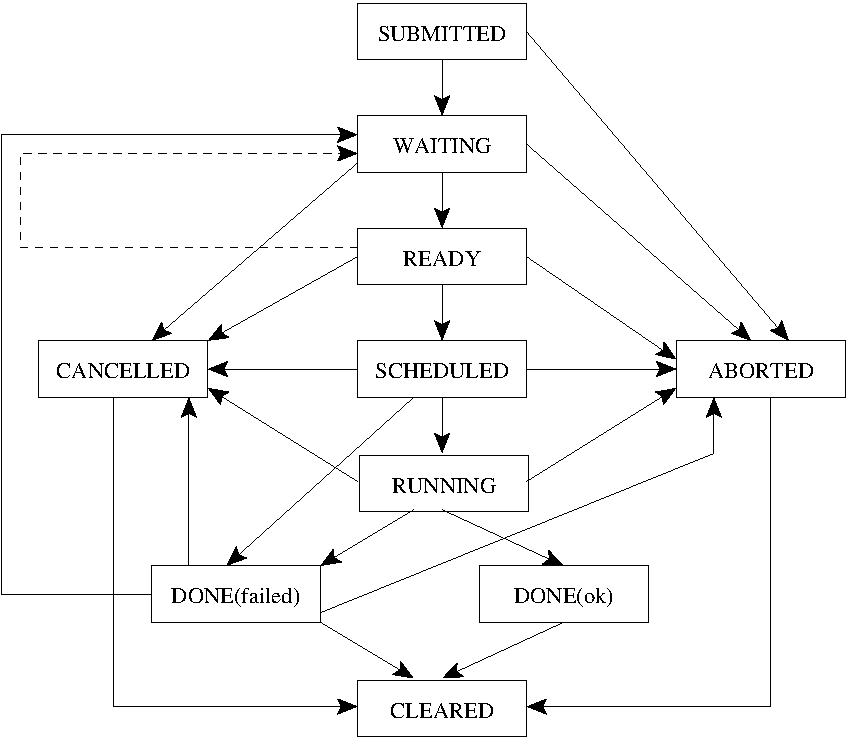
\includegraphics[width=.6\hsize]{images/wms2-jobstat}
\caption{\LB\ job state diagram}
\label{f:jobstat}
\end{figure}

% typ udalosti -> zmeny typu stavu
\LB\ defines a~\emph{job state machine} that is responsible for updating
the job state on receiving a~new event.
The logic of this algorithm is non-trivial; the rest of this section deals
with its main features.

Transitions between the job states happen on receiving events of particular
type coming from particular sources.
There may be more distinct events assigned to a~single edge of the state diagram.
For instance, the job becomes \emph{Scheduled} when it enters batch system
queue of a~Grid computing element.
The fact is witnessed by either \emph{Transfer/OK} event reported by 
the job submission service or by \emph{Accept} event reported by the computing
element. Receiving any one of these events (in any order) triggers the
state change.

% fault tolerance
This way, the state machine is highly fault-tolerant---it can cope with
delayed, reordered or even lost events.
For example, when a~job is in the \emph{Waiting} state and the \emph{Done}
event arrives, it is not treated as inconsistency but it is assumed that
the intermediate events are delayed or lost and the job state is switched
to the \emph{Done} state directly.

% udalosti nesou atributy, promitaji se do stavu 
The \LB events carry various common and event-type specific attributes,
\eg \emph{timestamp} (common) or \emph{destination} (\emph{Transfer} type).
The job state record contains, besides the major state identification,
similar attributes, \eg
an array of timestamps indicating when the job entered each state,
or \emph{location}---identification of the Grid component which is currently
handling the job.
Updating the job state attributes is also the task of the state machine,
employing the above mentioned fault tolerance---despite a~delayed event
cannot switch
the major job state back
it still may carry valuable information to update the job state attributes.

% typy jobu
Jobs monitored by \LB service may have different type. For gLite jobs, \LB supports
simple jobs and jobs representing \emph{set of jobs} -- \emph{DAGs} (with dependencies between 
subjobs described by direct acyclic graph) and \emph{collections} (without dependencies 
between subjobs). 
In these cases, subjobs are monitored in standard way, with one extensions - when job
status is changed, information is propagated also to the job representing corresponding 
collection or DAG.
Job representing collection or DAG can be used to monitor status of the set, including
information like how many subjobs is already finished etc.
Support for non-gLite jobs, namely for PBS or Condor systems, is described in section
\ref{sec:nonglite}.


\subsubsection{Event ordering}%
\label{evorder}

As described above, the ability to correctly order arriving events is
essential for the job state computation.
As long as the job state diagram was acyclic (which was true for the
initial WMS release), each event had its unique place in the expected sequence
hence event ordering could always be done implicitly from the
context.
However, this approach is not applicable once job resubmission
yielding cycles in the job state diagram was introduced.

Event ordering that would rely on timestamps assigned to events upon
their generation, assuming strict clock synchronization over the Grid,
turned to be a~naive approach.
Clocks on real machines are not precisely synchronized and there are no reliable
ways to enforce synchronization across administrative domains.

To demonstrate a problem with desynchronized clocks, that may lead to
wrong event interpretation, let us consider a~simplified example
in Tab.~\ref{t:cefail}.
%
\iffalse %stare
% usporadani udalosti -- seq. cisla
% priklad problemu
So far we assumed that the state machine is able to detect a~delayed event.
As the state diagram contains cycles, delay cannot be detected from the type
of the event only.
The simplest approach is relying on the event timestamps.
However, in the Grid environment one cannot assume strictly synchronized clocks.
Table~\ref{t:cefail} shows a~simplified example of the problem caused by delayed
clocks. 
\fi
%
\begin{table}[ht]
\begin{center}
\begin{tabular}{rlrl}
1.&WM: Accept&
6.&WM: Accept\\
2.&WM: Match $A$&
7.&WM: Match $B$\\
3.&WM: Transfer to $A$&
8.&WM: Transfer to $B$\\
4.&CE~$A$: Accept &
9.&CE~$B$: Accept \\
5.&CE~$A$: Run &
10.&CE~$B$: Run \\
\dots & $A$ dies\\
\end{tabular}
\end{center}
\caption{Simplified \LB events in the CE failure scenario}
\label{t:cefail}
\end{table}
%
We assume that the workload manager (WM) sends the job to a~computing element
(CE)~A, where it starts running but the job dies in the middle.
The failure is detected and the job is resubmitted back to the WM which sends it to CE~B then.
However, if A's clock is ahead in time and B's clock is correct (which
means behind the A's clock), the events in the right column are treated
as delayed. The state machine will interpret events incorrectly, assuming
the job has been run on B before sending it to A.
The job would always (assuming the A's events arrive before B's events to
the \LB) be reported as ``\emph{Running} at A'' despite
the real state should follow the \emph{Waiting} \dots \emph{Running} sequence.
Even the \emph{Done} event can be sent by B with a timestamp that says
this happened before the job has been submitted to A and the job state
will end with a discrepancy---it has been reported to finish on B while
still reported to run on A.

Therefore we are looking for a~more robust and general solution. We can
discover severe clock bias if the timestamp on an event is in a future
with respect to the time on an \LB server, but this is generally a dangerous
approach (the \LB server clock could be severely behind the real time).
We decided not to rely on absolute time as reported by timestamps, but to
introduce a kind of \emph{logical time} that is associated with the logic
of event generation.
The principal idea is arranging the pass through the job state 
diagram (corresponding to a~particular job life), that may include
loops, into an execution tree that represents the job history.
Closing a~loop in the pass through the state diagram corresponds
to forking a~branch in the execution tree.
The scenario in Tab.~\ref{t:cefail} is mapped to the tree in
Fig.~\ref{f:seqtree}.
The approach is quite general---any finite pass through any state
diagram (finite directed graph) can be encoded in this way.

\begin{figure}[ht]
\centering
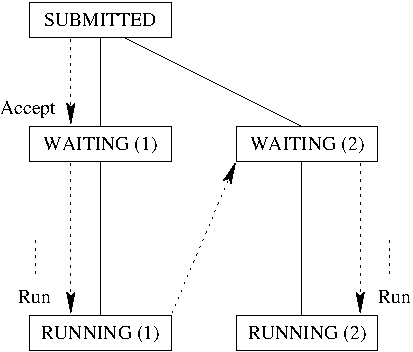
\includegraphics[scale=.833]{images/seqtree}
\caption{Job state sequence in the CE failure scenario, arranged into a~tree.
Solid lines form the tree, arrows show state transitions.}
\label{f:seqtree}
\end{figure}

Our goal is augmenting \LB events with sufficient information that
\begin{itemize}
 \item identifies uniquely a~branch on the execution tree, 
 \item determines the sequence of events on the branch, 
 \item orders the branches themselves, which means that it determines
   which one is more recent.  
\end{itemize}
If such information is available, the execution tree can be
reconstructed on the fly as the events arrive, and even delayed events
are sorted into the tree correctly.  An incoming event is considered
for job state computation only if it belongs to the most recent
branch.

The situation becomes even more complicated when 
the \emph{shallow resubmission} WM advanced feature is enabled.
In this mode WM may resubmit the job before being sure the previous attempt
is really unsuccessful, potentially creating multiple parallel instances
of the job.
The situation maps to several branches of the execution tree that
evolve really in parallel.
However, only one of the job instances becomes active (really running) finally;
the others are aborted.
Because the choice of active instance is done later, 
it may not correspond to the most recent execution branch.
Therefore, when an event indicating the choice of active instance arrives,
the job state must be recomputed, using the corresponding active branch
instead the most recent one.

Section~\ref{seqcode} describes the current implementation of event
ordering mechanism based on ideas presented here.

\subsubsection{Queries and notifications}\label{retrieve}

According to the GMA classification the user retrieves data from
the infrastructure in two modes, called
\emph{queries} and \emph{notifications} in~\LB.

Querying \LB is fairly straightforward---the user specifies query
conditions, connects to the querying infrastructure endpoint, and
receives the results. 
For ``single job'' queries, where jobid is known, the endpoint (the
appropriate \LB server) is inhered from the jobid.
More general queries must specify the \LB server explicitely,
and their semantics is intentionally restricted 
to ``all such jobs known here''.
We trade off generality for performance and reliability,
leaving the problem of finding the right query endpoint(s), the right
\LB servers, to higher level information and service-discovery services.

If the user is interested in one or more jobs, frequent polling of the
\LB server may be cumbersome for the user and creates unnecessary overload
on the sever. A notification subscription is therefore available,
allowing users to subscribe to receive notification whenever a~job 
starts matching user specified conditions.
Every subscription contains also the location of the user's
listener; 
successful subscription returns time-limited \emph{notification handle}.
During the validity period of the subscription, the \LB infrastructure
is responsible for queuing and reliable delivery of the notifications.
The user may even re-subscribe (providing the original handle) with different
listener location (\eg moving from office to home), and \LB re-routes
the notifications generated in the meantime to the new destination.
The \LB event delivery infrastructure is reused for the notification
transport.

\subsubsection{Local views}\label{local}
% motivace proxy

%As outlined in Sect.~\ref{reqs} 
WMS components are, besides logging
information into \LB, interested in querying this information back in order
to avoid the need of keeping per-job state information.
However, despite the required information is present in \LB,
the standard mode of \LB operation is not suitable for this purpose due
to the following reasons:
\begin{itemize}
\item Query interface is provided on the \LB component which gathers
events belonging to the same job but coming from different sources. 
Typically, this is a~remote service with respect to the event sources (WMS components).
Therefore the query operation is sensitive to any network failure that may
occur, blocking the operation of the querying service for indefinite time.
\item Due to the asynchronous logging semantics, there is a~non-zero time
window between successful completion of the logging call and the point in
time when the logged event starts affecting the query result.
This semantics may yield unexpected, seemingly inconsistent outcome. 
\end{itemize}

The problem can be overcome by introducing \emph{local view} on job data.
Besides forwarding events to
the server where events belonging to a~job are gathered from multiple sources,
\LB infrastructure can store the logged events temporarily
on the event source, and perform the processing described
in Sect.~\ref{evprocess}.
In this setup, the logging vs.\ query semantics can be synchronous---it is
guaranteed that a~successfully logged event is reflected in the result of
an immediately following query,
because no network operations are involved.
Only events coming from this particular physical node (but potentially
from all services running there) are considered, thus the locality of the view. 
On the other hand, certain \LB events are designed to contain redundant
information, therefore the local view on processed data (job state) 
becomes virtually complete on a~reasonably rich \LB data source like
the Resource Broker node.


\subsection{Current \LB implementation}
The principal components of the \LB service and their interactions
are shown in Figures~\ref{f:comp-gather} (gathering and transferring
\LB events) and~\ref{f:comp-query} (\LB query and notification services).

\begin{figure}[ht]
\centering
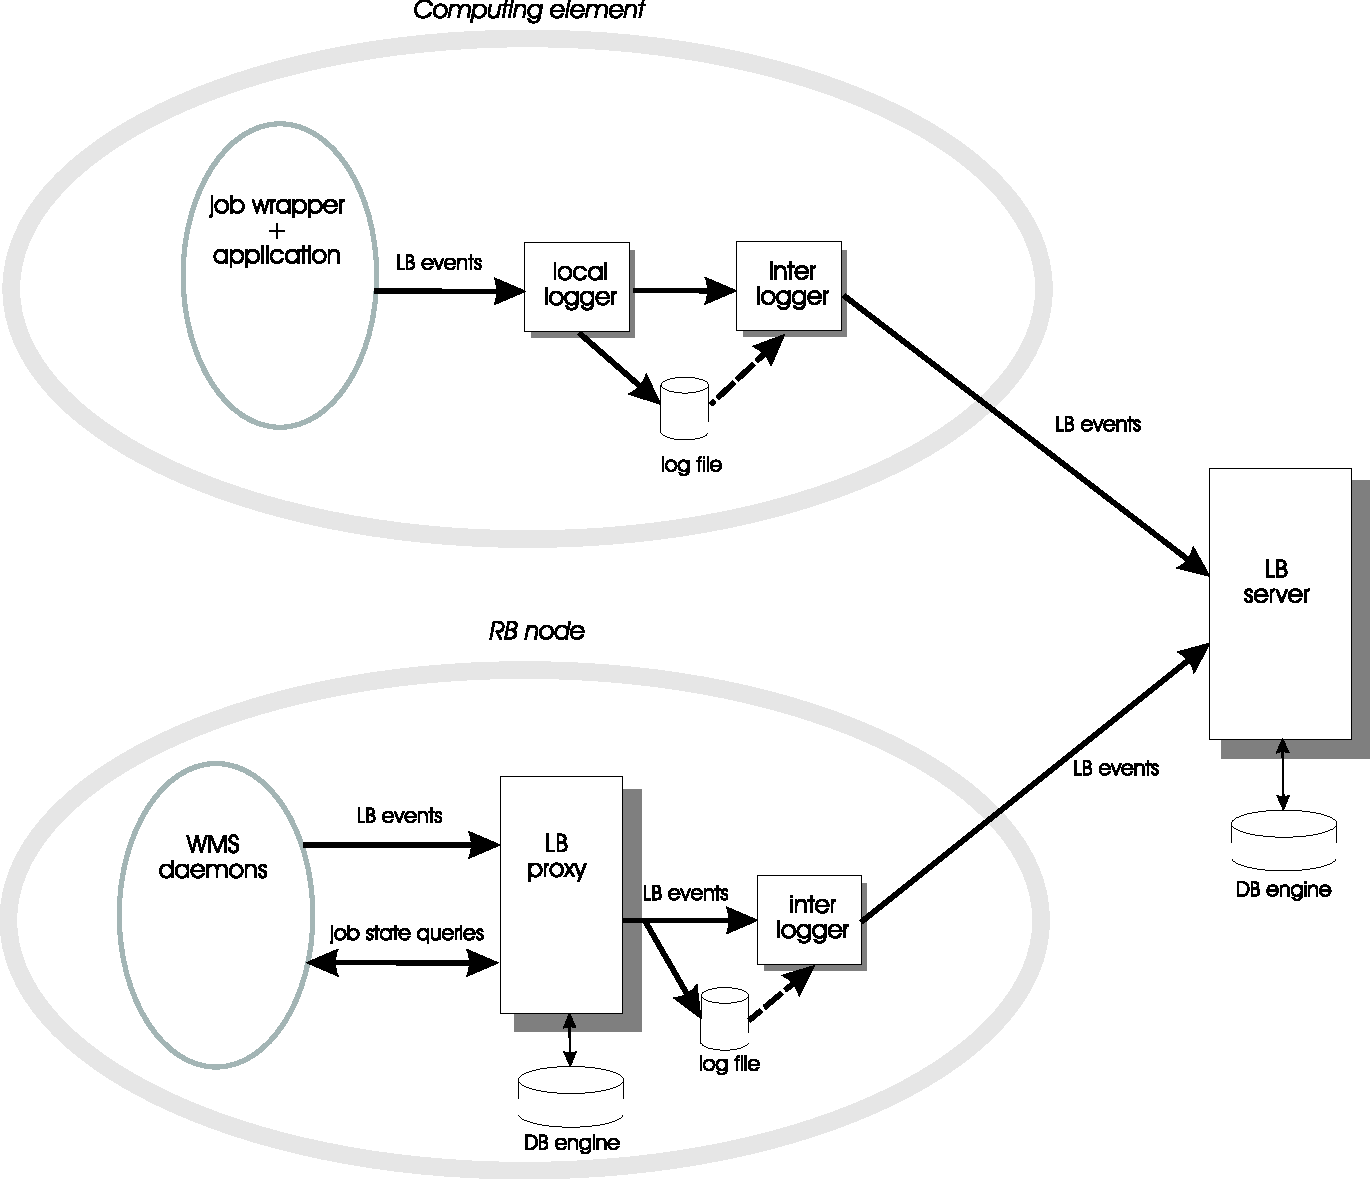
\includegraphics[scale=.5]{images/LB-components-gather}
\caption{\LB components involved in gathering and transferring the events}
\label{f:comp-gather}
\end{figure}

\input components

\subsubsection{Sequence codes for event ordering}%
\label{seqcode}

As discussed in Sect.~\ref{evorder}, sequence codes are used as logical
timestamps to ensure proper event ordering on the \LB server. The sequence code
counter is incremented whenever an event is logged and the sequence code must
be passed between individual Grid components together with the job control.
However, a single valued counter is not sufficient to support detection of
branch forks within the execution tree. When considering again the Computing
Element failure scenario described in Sect.~\ref{evorder}, there is no way to
know that the counter value of the last event logged by the failed CE A is 5
(see Table~\ref{t:cefail} on page~\pageref{t:cefail}). 

Therefore we define a~hierarchical \emph{sequence code}---an array of
counters, each corresponding to a~single Grid component class handling the job%
\footnote{Currently the following gLite components: Network Server, Workload
Manager, Job Controller, Log Monitor, Job Wrapper, and the application itself.}.
Table~\ref{t:cefail2} below shows the same scenario with a~simplified two-counter
sequence code. The counters correspond to the WM and CE component classes
and they are incremented when each of the components logs an event.
When WM receives the job back for resubmission, 
the CE counter becomes irrelevant (as the job control is on WM now),
and the WM counter is incremented again.

\begin{table}[ht]
\begin{center}
\begin{tabular}{rlrl}
1:x&WM: Accept&
4:x&WM: Accept\\
2:x&WM: Match $A$&
5:x&WM: Match $B$\\
3:x&WM: Transfer to $A$&
6:x&WM: Transfer to $B$\\
3:1&CE~$A$: Accept &
6:1&CE~$B$: Accept \\
3:2&CE~$A$: Run &
6:2&CE~$B$: Run \\
\dots & $A$ dies\\
\end{tabular}
\end{center}
\caption{The same CE failure scenario: hierarchical sequence codes.
``x'' denotes an undefined and unused value.}
\label{t:cefail2}
\end{table}

%Events on a~branch are ordered following the lexicographical order
%of the sequence codes.
%Branches are identified according to the WM counter as WM is 
%currently the only component where branching can occur.

The state machine keeps the current (highest seen) code for the job, 
being able to detect a~delayed event by simple lexicographic comparison
of the sequence codes.
Delayed events are not used for major state computation, then.
Using another two assumptions (that are true for the current
implementation):
\begin{itemize}
 \item events coming from a~single component arrive in order,
 \item the only branching point is WM,
\end{itemize}
it is safe to qualify events with lower WM counter (than the already
received one) to belong to inactive
branches, hence ignore them even for update of job state attributes.

\subsubsection{\LB data protection}
Events passed between the \LB components as well as the results of their
processing provide detailed information about the corresponding job and its
life and users obviously expect the job data provided by the \LB server to
be credible, reflecting the real jobs' operation on the Grid. Therefore, the
data must be based solely on authentic information generated by legitimate
grid components. The job data also provides information about user's
activities, which many users want to keep private. In order to provide a
sufficient level of security, the \LB infrastructure implements a security
mechanism that provides data protection and access control to the data.

All the \LB components communicate solely over secure channels whenever they
send data over a network. The TLS protocol~\cite{tls} is used for both mutual
authentication of the client and server and also encryption of the
communication. All the \LB components as well as the clients must possess a
digital certificate that they use to prove their identity. The \LB
infrastructure supports both standard X.509 certificates or proxy
certificates~\cite{proxycert} that are standard authentication mechanism in
the gLite environment. Depending on the server configuration and action
requested, the users may be required to present VOMS attributes in their
proxy certificates.

By default, access to information about a job is only allowed to the user
who submitted the job (\ie the job owner). The job owner can also assign an
access control list to his or job in the \LB specifying other users who are
allowed to read the data from \LB. The ACLs are represented in
the GridSite GACL format~\cite{gacl2} and are stored in the \LB database
along with the job information. The stored ACL are checked on each query
requesting the data. The ACLs are under control of the job owner, who can
add and remove entries in the ACL arbitrarily using the \LB API or
command-line tools (see~\ref{e:change-acl}). Each entry of an ACL can
specify either a user subject name, a name of a VOMS group, or an attribute
specified in the Full qualified attribute name format (the FQAN support is
only available in \LBnew). An ACL assigned to a job is returned as part of 
job status information.

Besides of using the ACLs, the \LB administrator can also specify a~set of
privileged users with access to all job records on a particular \LB server
(\emph{super-users}). These privileged users can \eg collect information on
usage and produce monitoring data based on the \LB information.

%Data trustworthiness - the events aren't signed, no real non-reputability or
%traceability of the event sources.


\subsection{User interaction}
\begin{figure}[ht]
\centering
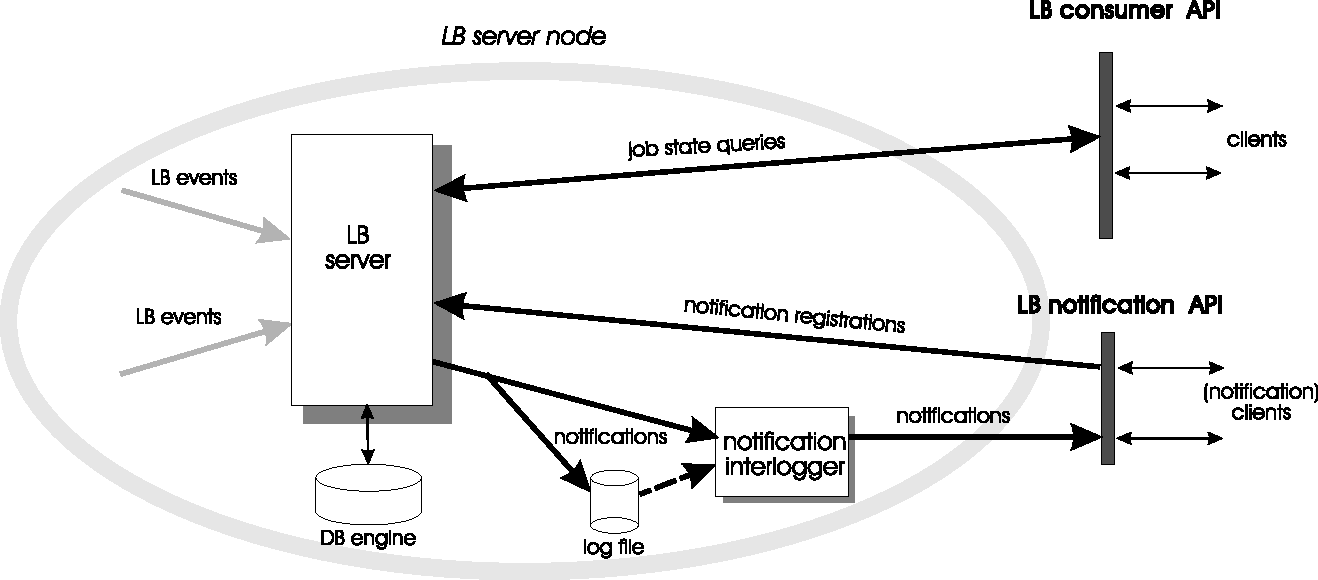
\includegraphics[scale=.5]{images/LB-components-query}
\caption{\LB queries and notifications}
\label{f:comp-query}
\end{figure}

So far we focused on the \LB internals and the interaction between its
components.
In this section we describe the interaction of users with the service.

\subsubsection{Event submission}
%implicitn� -- registrace jobu, syst�mov� ud�losti na middlewarov�ch komponent�ch
The event submission is mostly implicit,
\ie it is done transparently by the Grid middleware components
on behalf of the user.
Typically, whenever an important point in the job life is reached,
the involved middleware component logs an appropriate \LB event.
This process is not directly visible to the user.

A specific case is the initial registration of the job.
This must be done synchronously, as otherwise subsequent events logged for
the same job may be refused with a ``no such job'' error report. 
Therefore submission of a job to the WMS is the only synchronous event
logging that does not return until the job is successfully registered with
the \LB server.

% explicitn� -- user tagy, ACL
However, the user may also store information into the \LB explicitly
by logging user events---\emph{tags} (or annotations) of the
form ``name = value''.
Authorization information is also manipulated in this way. 

Description of tools for event submission and ACL manipulation 
can be found in Section \ref{s:lb-tools}.


\subsubsection{Querying information}
%\TODO{prejmenovat, aby v nazvy byly Queries}

From the user point of view, the information retrieval (\emph{query}) is the
most important interaction with the \LB service.

%dotazy na stav
The typical \LB usage are queries on the high-level job state information.
\LB supports not only single job queries, it is also possible to
retrieve information about jobs matching a specific condition.
The conditions may refer to both the \LB system attributes
and the user annotations. Rather complex query semantics can be
supported, \eg 
\emph{Which of my jobs annotated as ``apple'' or ``pear'' are already
scheduled for execution and are heading to the ``garden'' computing element?}
The \LB Developer's
Guide\cite{lbdg} provides a~series of similar examples of
complex queries.

%dotazy na ud�losti
As another option, the user may retrieve raw \LB events.
Such queries are mostly used for debugging, identification of repeating
problems, and similar purposes.
The query construction refers to event attributes rather
than job state.

The query language supports common comparison operators, and it allows
two-level nesting of conditions (logically \emph{and}-ed and \emph{or}-ed).
Our experience shows that it is sufficiently strong to cover most user
requirements while being simple enough to keep the query cost reasonable.
Complete reference of the query language can be found in~\LB Developer's Guide
\cite{lbdg}.

\subsubsection{Notifications}
The other mode of user interactions are the \LB notifications.

\LB infrastructure enables its users to be notified when something interesting happens on a \LB server
(typically job status change). It enables the user not to poll \LB server periodically to find changed
information, but confortably wait for server to inform the user.

User registers for notifications via notification client \verb'glite-lb-notify', described in Section
\ref{s:lb-notify}. 
Conditions under which the notification is sent can be specified. For example - job XY reaches status
DONE. In \LBold, one or more JOBID's are required in the condition and only a single occurence 
of a specific attribute is allowed among ANDed conditions. In \LBnew, more complex conditions are allowed.

The registration is then delivered to \LB server where it is stored.
At the same time, server generates a unique notification ID for the registration and returns it to the
user.

The registration exists only for limited amount of time. The validity is returned by \LB server together with
the notification ID when registering. During this period user can attach to server and receive notifications,
change conditions which triger notification, prolong validity of the registration, or remove the registration
from \LB server. 

While the registration is valid, user is able repeatably connect to \LB server from different places in the
network and continue receiving notifications associated with given notification ID. Notifications generated
during the time when user is connected are stored and waiting when user reconnects. 

\subsubsection{Caveats}
\LB is designed to perform well in the unreliable distributed Grid
environment.
An unwelcome but inevitable consequence of this design 
are certain contra-intuitive features in the system behavior,
namely:
\begin{itemize}
\item 
Asynchronous, possibly delayed event delivery may yield seemingly
inconsistent view on the job state \wrt\ information that is available
to the user via different channels.
\Eg the user may know that her job terminated because of monitoring the
application progress directly, but the \LB \emph{Done} events indicating
job termination are delayed so that \LB reports the job to be still
in the \emph{Running} state.

\item 
% sekven�n� ��sla -- �patn� �azen� ud�losti jsou ignorov�ny pro v�po�et stavu
Due to the reasons described in Sect.~\ref{evorder} \LB is rather sensitive
to event ordering based on sequence codes.
The situation becomes particularly complicated when there are multiple
branches of job execution.
Consequently the user may see an \LB event that is easily interpreted that
it should switch the job state, however, it has no effect in fact
because of being (correctly) sorted to an already inactive branch.

\item 
% purge -- data z~\LB\ zmiz�
\LB is not a~permanent job data storage. The data get purged from the
server on timeout, unrelated to any user's action.
Therefore, the \LB query may return ``no such job'' error message (or not
include the job in a list of retrieved jobs) even if the same previous
\LB query had no such problems.

\end{itemize}

\ludek{\subsection{Performance and scalability}
The \LB service was designed with performance and
scalability issues in mind. We have developed a series of tests of the
individual \LB components to measure the actual behavior under
stress conditions. These tests give us a good performance estimate of
the \LB service and help us identify and remove possible bottlenecks.

The testing itself is done by feeding the \LB components with events
prepared beforehand, using whatever protocol appropriate for the given
component. The feeding program uses a set of predefined events of a
typical job which we have chosen from the production \LB server
database. Timestamp is taken before the first event is sent, then the
feeding program begins sending events of individual jobs (the jobs are
all the same, the only difference is the jobid; the number of jobs used is
configurable). The tested component is instrumented in the source code
to break normal event processing at selected points (\eg discard
events immediately after being read to measure the input channel
performance, or discard events instead of sending them to the next
component, etc.). This segmentation of event processing enables to
identify places in the code which may slow down the event transfer. 
Optionally the events may be discarded by the next component in the
logical path. The last event of the last job is special termination
event, which is recognized when being discarded; then the second
timestamp is taken and the difference between the two gives us total
time necessary to pass given number of jobs through. 

Note that due to the asynchronous nature of the \LB service measuring for
example the time it takes to send given number of jobs does not give
us the required result, thus event (or job) throughput---when the
producer receives acknowledgment about successful send operation, it
is not guaranteed that the event passed through the component. 

The results shown in table~\ref{perf:results} give the overall
throughput components (events are discarded by the next component
on the path), with the exception of proxy, where the throughput to the
database is measured. It can be seen that the majority of code is fast
enough to handle even high event rates and that most components are up
to our goal to handle one million of jobs per day.  The first line
indicates how fast we are able to ``generate'' events in the feeding
program. 

\begin{table}[ht]
\begin{tabular}{l|r}
{\bf Component} & {\bf Job throughput (jobs/day)} \\
\hline
Test producer & 153,600,000 \\
Locallogger & 101,700 \\
Interlogger & 5,335,100 \\
Proxy & 1,267,110 \\
\end{tabular}
\caption{Performance testing results}
\label{perf:results}
\end{table}

During the performance testing we have identified two possible
bottlenecks:
\begin{itemize}
\item Opening connections and establishing SSL sessions is very
expensive operation. It hinders mainly the performance of locallogger,
because the current implementation uses one SSL session for
event.
\item Database operations. Storing events into database is expensive,
but inevitable; however we were able to optimize for example the
code checking for duplicated events.
\end{itemize}

In the current work we are addressing the issue of SSL operations by
introducing concept of SSL connection pools, which enables components
to reuse existing connections transparently without need to tear-down
and setup new SSL contexts. }

\subsection{Advanced use}

The usability of the \LB service is not limited to the simple tasks
described earlier. It can be easily extended to support real-time job
monitoring (not only the notifications) and the aggregate information
collected in the \LB servers is a valuable source of data used for post-mortem
statistical analysis of jobs and also the Grid infrastructure behavior.
Moreover, \LB data can be used to improve scheduling decisions.

\subsubsection{\LB and real time monitoring}
The \LB server is extended to provide quickly and without any substantial
load on the database engine the following data:
\begin{enumerate}
\item number of jobs in the system grouped by internal status
(\emph{Submitted}, \emph{Running}, \emph{Done},~\ldots),
\item number of jobs that reached final state in the last
hour,
\item associated statistics like average, maximum, and minimum time spent
by jobs in the system,
\item number of jobs that entered the WMS system in the last hour.
\end{enumerate}
\LB server can be regularly queried to provide this data to give an
overview about both jobs running on the Grid and also the behavior of the
Grid infrastructure as seen from the job (or end user) perspective.
Thus \LB\ becomes a~data source for various real-tim Grid monitoring tools.

\subsubsection{R-GMA feed}
The \LB server also supports streaming the most important data---the job
state changes---to another monitoring system. It works as the
notification service, sending information about job state changes to
a~specific listener that is the interface to a monitoring interface.
As a~particular example of such a generic service, the R-GMA feed component
has been developed. It supports sending job state changes to
the R-GMA infrastructure that is part of the Grid monitoring
infrastructure used in the EGEE Grid.

Currently, only basic information about job state changes is provided
this way, taking into account the security limitation of the R-GMA. 

\subsubsection{\LB Job Statistics}
Data collected within the \LB servers are regularly purged, complicating
thus any long term post-mortem statistical analysis. Without a Job
Provenance, the data from the \LB must be copied in a controlled way and
made available in an environment where even non-indexed queries can be
asked. 

Using the \LB Job Statistics tools, one dump file per job is created 
when the job reaches a~terminal state. These dump files can be
further processed to provide and XML encoded Job History Record%
\footnote{\url{http://egee.cesnet.cz/en/Schema/LB/JobRecord}} that
contains all the relevant information from the job life. The Job History
Records are fed into a statistical tools to reveal interesting information
about the job behavior within the Grid.

This functionality is being replaced by the direct download of all the
relevant data from the Job Provenance.

\subsubsection{Computing Element reputability rank}
\label{s:ce-rank}
Production operation of the EGEE middleware showed
that misbehaving computing elements may have significant impact on
the overall Grid performance.
The most serious problem is the ``black hole'' effect---a~CE that
accepts jobs at a~high rate but they all fail there.
Such CE usually appears to be free in Grid information services
so the resource brokers keep to assign further jobs to it.

\LB data contain sufficient information to identify similar problems.
By processing the incoming data the information
was made available as on-line auxiliary statistics like
rate of incoming jobs per CE, rate of job failure, average duration of job etc.
The implementation is lightweight, allowing very high query rate.
On the RB the statistics are available as ClassAd
functions, allowing the user to specify that similarly misbehaving
CE's should be penalized or completely avoided
when RB decides where jobs get submitted.


\subsubsection{Non-gLite event sources}
\label{sec:nonglite}

\LB has been enhanced to support also non-gLite events, namely events from PBS
or Condor batch systems \cite{hpdc07}. These events are handeled differently from gLite events,
for a complete list of the PBS and Condor events see Appendix \ref{a:events}. 
Since job states in the batch system slightly differ from the states of a job
defined in \LB (see also Appendix \ref{a:jobstat}), events are processed separately
from gLite events. Both PBS and Condor events has its own state machine that processes the
events and determines the now state of the job.

Recently, there were also attempts to use \LB system to transport different types of events: 
Certificate Revocation Lists or syslog messages. For a detailed description see 
\cite{LB4CRL}.



\subsection{Service Architecture}

Within the gLite WMS, upon creation
 each job is assigned a~unique, virtually non-recyclable
\emph{job identifier} (JobId) in an~URL form.
The server part of the URL designates the \emph{bookkeeping server} which
gathers and provides information on the job for its whole life.

High level view on the \LB\ architecture is shown in Fig.~\ref{fig-arch}
on page~\pageref{fig-arch}.

\LB\ tracks jobs in terms of \emph{events} (\eg\ \emph{Transfer} from a~WMS
component to another one, \emph{Run} and \emph{Done} when the jobs starts
and stops execution, \dots).
Each event type carries its specific attributes.
The entire architecture is specialized for this purpose and is job-centric\Dash
any event is assigned to a~unique Grid job.

\subsubsection{Event delivery and storage}
The events are gathered from various WMS components by the
\emph{\LB\ producer library}
and passed on to the \emph{locallogger} daemon,
running physically close to avoid
any sort of network problems.
The locallogger's task is storing the accepted event in a~local disk file.
Once it's done, confirmation is sent back and the logging library call
returns, reporting success.
Consequently, logging calls have local, virtually non-blocking semantics.

Further on, event delivery is managed by the \emph{interlogger} daemon.
It takes the events from the locallogger (or the disk files on crash recovery),
and repeatedly tries to deliver them to the destination
bookkeeping server (known from the JobId) until it succeeds finally.
Therefore the entire event delivery is highly reliable.
However, in the standard mode described so far it is asynchronous
(there is a~synchronous mode for special usage not discussed here)
there is no direct way for the caller to see whether an event has been
already delivered.
Our experience shows that the semantics is suitable in the prevailing number
of cases while being the most efficient in the erratic Grid environment.

The bookkeeping server processes the incoming events
to give a~higher level view
on the job states (\eg\ \emph{Submitted, Running, Done}),
each having an appropriate set of attributes again.
\LB\ provides a~public interface (Sect.~\ref{query-C})
to retrieve them via synchronous queries.

Further on, upon each event delivery to the \LB\ server the new computed 
job state is matched against the set of registered requests for notification.
If some of them match, special events\Dash\emph{notifications} are generated
and passed to a~modified 
\emph{notification interlogger}.
It takes over the notification from LB server, stores it into file and
periodically tries to deliver it to the address where the corresponding
notification client is listening.
If the user changes this address (IP or port) 
\LB\ server instructs the notification interlogger to change 
the destination of possible pending notifications.

\subsubsection{Queries}
\label{arch-queries}
One part of the \LB\ interface is the query API (Sect.~\ref{query-C}).
Two types of queries are supported\Dash\emph{job queries} which return
one or more jobs, including a~detailed description of their states,
and \emph{event queries} returning the raw \LB\ events.
In general, job queries are used to track normal life of jobs,
event queries are used mostly for tracing abnormal behaviour. 

Each query is formed of several conditions (\eg\ concrete jobid's,
owner of jobs, particular job state etc.).
The \LB\ library formats the conditions into a~query message, passes it to
the server, and waits for the response which is passed to the user
synchronously.

\subsubsection{Notifications}
\label{notification}
On the contrary, the notification API (Sect.~\ref{notify-C}) allows
the user to 
register for notifications. These are delivered to the listening
client asynchronously, when the particular event (a~change of job status
typically) occurs.
The main purpose of this \LB\ functionality is avoiding unnecessary load
on the \LB\ server serving many repeated queries (polling) with the same
result most of the time.

Using a~notification client (program that uses LB client
API to handle notifications) the user registers with a~\LB\ server
to receive notifications. 
She  must specify conditions under which the
notification is sent. These conditions are a~subset of the conditions
available for synchronous queries (Sect.~\ref{arch-queries}).
Currently due to implementation constraints, one
or more jobid's are required among the conditions and only
a~single occurrence of a~specific attribute is allowed. The registration is 
sent to the \LB\ server in the same way as synchronous queries,
and stored there.
In response, the server generates a~unique notification ID which is used
by the user to refer to this notification further on.
The user may
change conditions which trigger notification, prolong validity of
the registration, remove the registration from LB server,
or even change the destination of notifications, \ie\ the address where
a~client listens for notifications.

The registration is soft-state; it exists only for limited amount of time. The
validity is returned by LB server together with notification ID.

While the registration is valid, 
the user may stop the notification client and launch another, even
on a~different machine.
Notifications generated during the time when there was no client listening
for them are kept by the notification interlogger.
Once a~new listening address is announced to the
server, the pending notifications are delivered. 

\endinput

\subsection{Security and Access Control}

The \LB\ infrastructure ensures high level of security for information it
processes. All the \LB\ components communicate solely over authenticated
connections and users who query the \LB\ server also must authenticate properly
using their PKI certificates. All messages sent over the network are encrypted
and their content is not accessible to unauthorized people.

By default, information about a job stored in the \LB\ server is only available
to the user who submitted the job, i.e. the job owner.  Besides this default
functionality, the \LB\ server also allows the job owner to share job
information with another users. Each job can be assigned an access control list
(ACL) that specifies another users who are also allowed to access the job
information. The management of ACL's is entirely under control of the job owner
so she can modify the ACL arbitrarily, specifying the set of users who have
access to the job information. The users in the ACL's can be specified using
either the subject names from their X.509 certificates or names of VOMS groups.

Current ACL for a job is returned as part of the job status information
returned by the \verb'glite-job-status' command. The commands output ACL's in
the original XML format as specified by GACL/GridSite. 

Example of an ACL:
\begin{verbatim}
<?xml version="1.0"?><gacl version="0.0.1">
   <entry>
      <voms-cred><vo>VOCE</vo><group>/VOCE</group></voms-cred>
      <allow><read/></allow>
   </entry>
   <entry>
      <person><dn>/O=CESNET/O=Masaryk University/CN=Daniel Kouril</dn></person>
      <deny><read/></deny>
   </entry>
</gacl>
\end{verbatim}

This ACL allows access to all people in the VOMS group /VOCE in virtual
organization VOCE, but denies access to user Daniel Kouril (even if he was a
member of the /VOCE group).

The job owner herself is not specified in the ACL as she is always allowed to
access the information regardless the content of the job ACL.

An ACL for a job can be changed using the \verb'glite-lb-logevent' command-line
program, see section~\ref{change_acl}.

%provided in the example subdirectory. In order to use change\_acl, the \LB\
%daemons locallogger and interlogger must be running. The usage of the command
%is as follows:
%
%\LB\ server configuration
%In order to support the VOMS groups in the ACL's,
%glite_lb_bkserverd must be able to verify client's VOMS proxy certificate using
%a trusted VOMS service certificate stored on a local disk. Default directory
%with trusted VOMS certificates is /etc/grid-security/vomsdir, another location
%can be specified using by either the -V option to glite_lb_bkserverd or setting
%the VOMS_CERT_DIR environment variable.

\endinput

\subsection{Interactions with other Services}

The main \LB\ functionality is keeping track of jobs managed by
the Workload Management System otherwise.
Therefore its basic usage is done internally by the WMS components.
However, the query and notification interface is completely available
to user-level applications. Upto limited extent (two event types)
this holds for the event-logging interface too.

\subsubsection{Event sources}
\LB\ events are generated by the following WMS components:
\begin{description}
\item[User Interface] registers the job with \LB\ and provides details
on transfer of the job to the resource broker.
\item[Resource Broker,] consisting of several WMS components,
logs various events as the job is passed among these components, 
as well as other important job-related information (\eg\ the chosen
destination Computing Element).
\item[Computing Element,] via the Job Wrapper script, provides the immediate
information on job execution.
\end{description}
Besides these WMS components the job payload may also log UserTag events
(see Sect.~\ref{log_usertag}) containing arbitrary user information.

Checkpointable jobs also use \LB\ to keep track of the job progress.
This is done internally by the checkpoint support library.

Finally, changes of job access control lists are done by logging
another event. This may be done directly by the user or using the WMS
user interface.

\subsubsection{Queries}

The \LB\ queries with a~user-visible output
are executed from within WMS User Interface
commands glite-job-status and glite-job-logging-info.

Besides those several WMS components use \LB\ internally to query
information on job status which is relevant for their processing.

\subsubsection{Notifications}

Notifications on job state change are used by WMS GUI 
to monitor the state of jobs periodically.

\subsubsection{Component and Interaction Diagrams}
% \todo{nekdy priste}
% To help understanding the service a set of component and interaction
% diagrams might help. This section is not mandatory.

\begin{figure}[h]
\centering
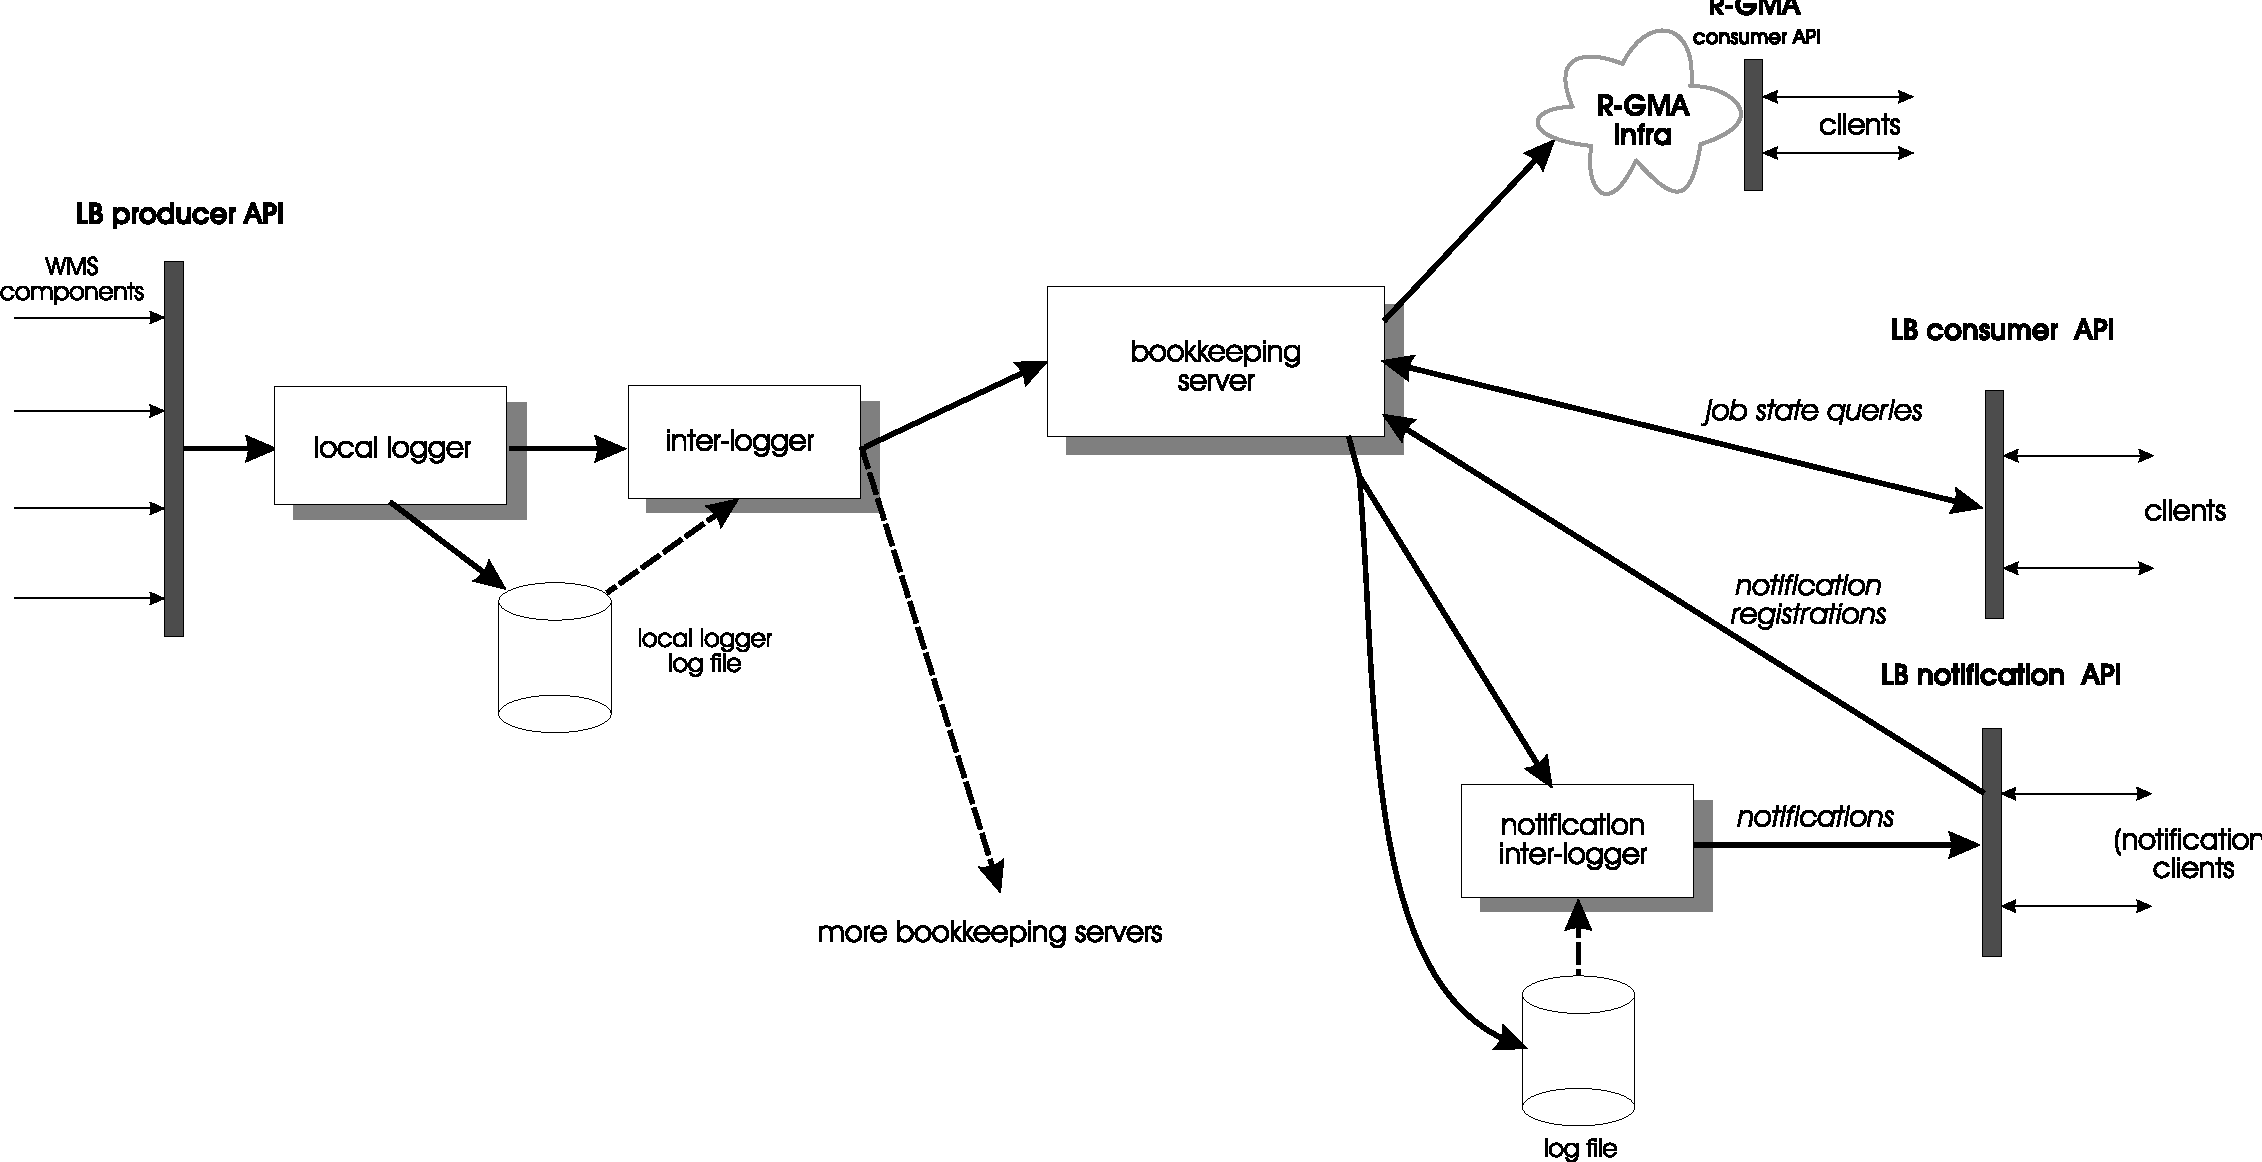
\includegraphics[width=.8\hsize]{logging-arch-notif}
\caption{Overview of the \LB\ architecture}
\label{fig-arch}
\end{figure}


\endinput


\newpage
\section{Quickstart Guide}
% The quickstart guide should explain in simple terms and with examples
% how a user is supposed to achieve the most common usecases. E.g. how
% to submit and cancel a job, how to receive a job's output. How to
% create a grid file, move it around, locate it, and delete it. How to
% monitor the progress on an application etc.

\subsection{Command-Line Tools}
This section describes usage of event-logging \LB\ command in the two
cases which are ment for the end-user: adding a~user description (tag)
to a~job, and changing a~job access control list.

\subsubsection{Logging a UserTag event}
\label{log_usertag}


User tag is an arbitrary ``name=value'' pair with which the user can 
assign additional information to a job. Further on, LB can be queried
based also on values of user tags.
% (see Sect.~\ref{tag-query}).

In order to add user tag for a job a special event \verb+UserTag+ is used. This
event can be logged by the job owner using the glite-lb-logevent command (see also
sec.\ref{cmdln_interface}). Here we suppose the command is used from user's running
 application because a correct setting of environment variables needed by 
the command is assured.

General template for adding user tag is as follows:

\begin{verbatim}
glite-lb-logevent -s Application -e UserTag    \
        -j <job_id>                         \
        -c <seq_code>                       \
        --name <tag_name>                   \
        --value <tag_value>
\end{verbatim}

where

\begin{tabularx}{\textwidth}{lX}
\verb'<job_id>'    & specifies the job to change \\
\verb'<seq_code>'   & specifies the sequence code returned by previous call
			of verb 'glite-lb-logevent'\\
\verb'<tag_name>'    & specifies the name of user tag\\
\verb'<tag_value>' & specifies the value of user tag\\
\end{tabularx}

The user application is always executed from within a JobWrapper script (part of Workload Management System \cite{WMS}). The wrapper  sets the  appropriate \verb'JobId' in the environment variable \verb'GLITE_WMS_JOBID'. The user should pass this value to the -j option of glite-lb-logevent.  Similarly, the wrapper sets an initial value of the event sequence code in the environment variable \verb'GLITE_WMS_SEQUENCE_CODE'.

If the user application calls glite-lb-logevent just once, it is sufficient to pass this value to the -c option.  However, if there are more  subsequent calls,  the  user is responsible for capturing an updated sequence code from the stdout of glite-lb-logevent and using it in subsequent calls.  The \LB\ design requires the sequence codes in  order  to  be able to sort events correctly while not relying on strictly synchronized clocks.  

The example bellow is a job consisting of 100 phases.  A user tag phase is used to log the phase  currently  being executed.  Subsequently, the user may monitor execution of the job phases as a part of the job status returned by \LB.

\begin{verbatim}
  #!/bin/sh

  for p in `seq 1 100`; do

  # log the UserTag event
  GLITE_WMS_SEQUENCE_CODE=`glite-lb-logevent -s Application
    -e UserTag
    -j $GLITE_WMS_JOBID -c $GLITE_WMS_SEQUENCE_CODE
    --name=phase --value=$p`

  # do the actual computation here
  done
\end{verbatim}



\subsubsection{Changing Job Access Control List}
\label{change_acl}
\subsubsection{Example: Changing Job Access Control List}
\label{e:change-acl}

In order to change the Access Control List (ACL) for a job, a special event
\verb'ChangeACL' is used. This event can be logged by the job owner using the
\verb'glite-lb-logevent' command (see also Sect.~\ref{glite-lb-logevent}).
The general template for changing the ACL is as follows:

\begin{verbatim}
glite-lb-logevent -e ChangeACL -s UserInterface -p -j <job_id>
        --user_id <user_id>                                             
        --user_id_type <user_id_type>                                   
        --permission READ
        --permission_type <permission_type> --operation <operation>
\end{verbatim}

where

\begin{tabularx}{\textwidth}{>{\texttt}lX}
\verb'<job_id>'    & specifies the job to change access to\\
\verb'<user_id>'   & specifies the user to grant or revoke permission. The
               parameter can be either an X.500 name
               (subject name), a VOMS group (of the form VO:Group), or a Full
               qualified attribute name (FQAN). \\
\verb'<user_id_type>' & indicates the type of the user\_id given above.
               \verb'DN', \verb'GROUP', and \verb'FQAN' can be given to
               specify X.500 name, VOMS group, or FQAN, respectively \\
\verb'<permission>' & ACL permission to change, currently only \verb'READ' is
               supported. \\
\verb'<permission_type>' & Type of permission requested. \verb'ALLOW' or
               \verb'DENY' can be specified. \\
\verb'<operation>' & Operation requested to be performed with ACL. \verb'ADD'
               or \verb'REMOVE' can be specified. \\
\end{tabularx}

Adding a user specified by his or her subject name to the ACL (\ie granting
access rights to another user):

\begin{verbatim}
glite-lb-logevent -e ChangeACL -s UserInterface -p -j <job_id>          \
        --user_id '/O=CESNET/O=Masaryk University/CN=Daniel Kouril'     \
        --user_id_type DN --permission READ --permission_type ALLOW     \
        --operation ADD
\end{verbatim}


Removing a user specified by his or her subject name from the ACL (\ie
revoking access right to another user):

\begin{verbatim}
glite-lb-logevent -e ChangeACL -s UserInterface -p -j <job_id>          \
        --user_id '/O=CESNET/O=Masaryk University/CN=Daniel Kouril'     \
        --user_id_type DN --permission READ --permission_type ALLOW     \
        --operation REMOVE
\end{verbatim}


Adding a VOMS attribute to the ACL:

\begin{verbatim}
glite-lb-logevent -e ChangeACL -s UserInterface -p -j <job_id>          \
        --user_id '/VOCE/Role=Administrator' --user_id_type FQAN        \
        --permission READ --permission_type ALLOW                       \
        --operation ADD
\end{verbatim}


Note that \LBold supported only using VOMS group names, not full FQANs,
whose support has been introduced only in \LBnew. \LBold also did not
allowed the users to use symbolic names for the values specifying ACL
setting and integers must be used instead. For example, to grant access
right on a \LBold server one has to use following syntax:

\begin{verbatim}
glite-lb-logevent -e ChangeACL -s UserInterface -p -j <job_id>          \
        --user_id '/O=CESNET/O=Masaryk University/CN=Daniel Kouril'     \
        --user_id_type 0 --permission 1 --permission_type 0 --operation 0
\end{verbatim}



%% \subsection{\LB Producer API}
%% \todo{honik}
%% This API is not public at the moment, it may change later.
%% % -*- mode: latex -*-

\section{\LB\ Logging (Producer) API}
\label{ProdOverview}
The \LB\ logging API (or producer API) is used to create and deliver
events to the \LB\ server and/or proxy, depending on the function
used:

\begin{table}[h]
\begin{tabularx}{\textwidth}{lX}
\bf Function & \bf Delivered to \\
\hline
\small\verb'edg_wll_LogEvent(...)' & asynchronously through
locallogger/interlogger to the \LB\ server \\
\small\verb'edg_wll_LogEventSync(...)' & synchronously through
locallogger/interlogger to the \LB\ server \\
\small\verb'edg_wll_LogEventProxy(...)' & through \LB\ proxy to the \LB\ server \\
\small\verb'edg_wll_Register*(...)' & directly to both \LB\ server and proxy \\
\small\verb'edg_wll_ChangeACL(...)' & directly to the \LB\ server \\
\end{tabularx}
\end{table}

These general functions take as an argument event format (which
defines the ULM string used) and variable number of arguments corresponding
to the given format. For each defined event there is predefined format
string in the form \verb'EDG_WLL_FORMAT_'\textit{EventType}, \eg\
\verb'EDG_WLL_FORMAT_UserTag', as well as three convenience functions
\verb'edg_wll_LogUserTag(...)', \verb'edg_wll_LogUserTagSync(...)',
\verb'edg_wll_LogUserTagProxy(...)'. 

For most developers (\ie\ those not developing the WMS itself) the
\verb'edg_wll_LogUserTag*(...)' and \verb'edg_wll_ChangeACL(...)' are
the only functions of interest.

\subsection{Call semantics}
\LB producer calls generally do not have transaction semantics, the
query following succesful logging call is not guaranteed to see
updated \LB server state. The typical call -- loging an event -- is
returned immediatelly and the success of the call means that the first
\LB infrastructure component takes over the event and queues it for
delivery. If you require transaction semantics, you have to use
synchronous \verb'edg_wll_LogEventSync(...)' call. 

The \LB proxy on the other hand provides a \emph{local view}
semantics, events logged into proxy using
\verb'edg_wll_LogEventProxy(...)' are guaranteed to by accessible by
subsequent queries \emph{on that proxy}.

Job registrations are all synchronous.

\subsection{Header files}

\begin{table}[h]
\begin{tabularx}{\textwidth}{>{\tt}lX}
glite/lb/producer.h & Prototypes for all event logging functions. \\
\end{tabularx}
\end{table}

\subsection{Context parameters}
The following table summarizes context parameters relevant to the
event logging. If  parameter is not set in the context explicitly, the
\LB\ library will search for value of corresponding environment
variable. The symbolic C names should be prepended with
\verb'EDG_WLL_PARAM_' prefix, \ie\ \verb'EDG_WLL_PARAM_HOST'.

\begin{table}[h]
\begin{tabularx}{\textwidth}{llX}
{\bf C name} & {\bf Env. variable} & {\bf Description} \\
\hline
\small\verb'HOST' & & Hostname that appears as event origin. \\
\small\verb'SOURCE' & & Event source component. \\
\small\verb'DESTINATION' & \small\verb'GLITE_WMS_LOG_DESTINATION' & Hostname of machine running
locallogger/interlogger. \\
\small\verb'DESTINATION_PORT' & \small\verb'GLITE_WMS_LOG_DESTINATION' & Port the locallogger is listening
on. \\
\small\verb'LOG_TIMEOUT' & \small\verb'GLITE_WMS_LOG_TIMEOUT' & Logging timeout for asynchronous
logging. \\
\small\verb'LOG_SYNC_TIMEOUT' & \small\verb'GLITE_WMS_LOG_SYNC_TIMEOUT' & Logging timeout for synchronous
logging. \\
\small\verb'LBPROXY_STORE_SOCK' & \small\verb'GLITE_WMS_LBPROXY_STORE_SOCK' & \LB\ Proxy store socket path (if
logging through \LB\ Proxy) \\
\small\verb'LBPROXY_USER' & \small\verb'GLITE_WMS_LBPROXY_USER' & Certificate subject of the user (if
logging through \LB\ proxy).
\end{tabularx}
\end{table}
The \verb'GLITE_WMS_LOG_DESTINATION' environment variable contains
both locallogger host and port separated by colon (\ie\ ``host:port'').

\subsection{Return values}
The logging functions return 0 on success and one of {\texttt EINVAL,
ENOSPC, ENOMEM, ECONNREFUSED, EAGAIN} on error. If {\texttt EAGAIN} is
returned, the function should be called again to retry the delivery;
it is not guaranteed, however, that the event was not delivered by the
first call. Possibly duplicated events are discarded by the \LB\
server or proxy.

The synchronous variants of logging functions can in addition return
\verb'EDG_WLL_ERROR_NOJOBID' or \verb'EDG_WLL_ERROR_DB_DUP_KEY'.

\subsection{Logging events}
In this section we will give an example how to log an UserTag event to
the \LB.

First we have to include neccessary headers:
\lstinputlisting[firstline=8,lastline=10]{prod_example1.c}

Initialize context and set parameters:
\lstinputlisting[firstline=61,lastline=84]{prod_example1.c}

\TODO{proper setting of sequence codes}
\lstinputlisting[firstline=86,lastline=91]{prod_example1.c}

Log the event:
\lstinputlisting[firstline=93,lastline=107]{prod_example1.c}

The \verb'edg_wll_LogEvent()' function is defined as follows:
\begin{lstlisting}[numbers=none]
extern int edg_wll_LogEvent(
        edg_wll_Context context,
        edg_wll_EventCode event,
        char *fmt, ...);
\end{lstlisting}
If you use this function, you have to provide event code, format
string and corresponding arguments yourself. The UserTag event has
only two arguments, tag name and value, but other events require more
arguments. 

Instead of using the generic \verb'edg_wll_LogEvent()', we could also
write:
\begin{lstlisting}[firstnumber=92]
err = edg_wll_LogUserTag(ctx, name, value);
\end{lstlisting}

\subsection{Java binding}



\subsection{\LB\ Querying API}
%\todo{valtri}
% -*- mode: latex -*-

\section{\LB\ Querying (Consumer) API}

\label{ConsOview}

\subsection{Query Language}

\subsection{C Language Binding}

\subsubsection{Call Semantics}

When the item count returned by \LB\ server exceeds the defined limits, the E2BIG error occur.
There are two limits\,---\,the server and the user limit. The user defined limit may be set in
the context at the client side in the following way:

\subsubsection{Header Files}
\begin{table}[h]
\begin{tabularx}{\textwidth}{>{\tt}lX}
glite/lb/consumer.h & Prototypes for all query functions. \\
\end{tabularx}
\end{table}

\subsubsection{Context Parameters}
\begin{itemize}
	\item{EDG\_WLL\_QUERYRES\_NONE}\,---\,No results are returned.
	In this case an E2BIG error acts like a hard error.
	\item{EDG\_WLL\_QUERYRES\_LIMITED}\,---\,A result contains at most ``limit'' item count.
	In this case an E2BIG error acts like a soft error.
	\item{EDG\_WLL\_QUERYRES\_ALL}\,---\,All results are returned and limits has no effect.
	This option is available only in special cases such as ``user jobs query'' and 
	the ``job status query''. Otherwise the EINVAL error is returned.
\end{itemize}
Default value is EDG\_WLL\_QUERYRES\_NONE.

\subsubsection{Return Values}
\LB\ server returns errors which are classified as hard and soft errors.
The main difference between these categories is that in the case of soft
errors results may still be returned.
The authorization errors belong to
``soft error'' sort. Hard errors are typically all unrecoverable errors like ENOMEM.

The E2BIG error may fall into both categories depending on the setting of
another context parameter, EDG\_WLL\_PARAM\_QUERY\_RESULTS.
It may take the following values:


\subsubsection{Job Queries}

The simplest case corresponds to the situation when an exact job ID
is known and the only information requested is the job status. The job ID
format is described in~\cite{djra1.4}.
The following example shows 
all the relevant structures and API calls to retrieve status information
about a job with the ID\\
\texttt{https://lhun.ics.muni.cz:9000/OirOgeWh\_F9sfMZjnIPYhQ}.

The first function call in this example initializes the \LB\ context\,---\,variable
\texttt{ctx}\,---\,which is necessary for later use. The most important part
of this code fragment is the \texttt{jc} variable setting.
Variable \texttt{jc} is a list of conditions terminated with the 
\texttt{EDG\_WLL\_QUERY\_ATTR\_UNDEF} item.
In this example it contains the only data item\,---\,the job ID
(in its parsed form).

If \texttt{edg\_wll\_QueryJobs()} is successful, returned results are available 
in the \texttt{statesOut} variable. This variable contains an array of job states\,---\,
in this example state of a given job.

The code also shows a~complete handling of returned errors as well as memory
management\,---\,deallocation of data that are not needed anymore.
\emph{For the sake of simplicity such code is not included in the examples
in the rest of this document.}

%\partitle{All user's jobs}
\label{JQ-auj}

\TODO{Update the example so that it is really working}

The simple query example is a request for all user's jobs. Another
condition type, \\
\texttt{EDG\_WLL\_QUERY\_ATTR\_OWNER}, is used in this case, with the 
value field filled with a user name. You can found this example in client module, file \texttt{job\_status.c}.

\begin{verbatim}
  #include <glite/lb/consumer.h>
  ...
  edg_wll_Context     ctx;    
  edg_wll_QueryRec    jc[2];
  edg_wll_JobStat    *statesOut = NULL;
  edg_wlc_JobId      *jobsOut = NULL;
  ...
  jc[0].attr = EDG_WLL_QUERY_ATTR_OWNER;
  jc[0].op = EDG_WLL_QUERY_OP_EQUAL;
  jc[0].value.c = NULL;
  jc[1].attr = EDG_WLL_QUERY_ATTR_UNDEF;
  edg_wll_QueryJobs(ctx, jc, 0, &jobsOut, &statesOut);
  ...
\end{verbatim}

The value of the \texttt{attr} field which specifies job owner
could be set to \texttt{NULL} meaning the authenticated user.
Obtained results may differ according to the security level, e.g. with strong security
context only information about jobs of the specified user are returned
(in general info about all jobs a user is authorized to retrieve should be
returned).

The query may return either a~list of job ID's or a~list of job states or both,
depending on the parameters \texttt{jobsOut} and \texttt{statesOut}.
If either is NULL the corresponding list is not retrieved.

Developers should keep in mind that the output of such a query could be really huge.
\par

The following examples demonstrates how \texttt{edg\_wll\_QueryJobs()} combines 
the given conditions in a logical conjugation.

%\partitle{Running jobs}
\label{JQ-rj}

If all (user's) running jobs are to be retrieved the following code can
be used.
\begin{verbatim}
  #include <glite/lb/consumer.h>
  ...
  edg_wll_Context     ctx;    
  edg_wll_QueryRec    jc[3];
  edg_wll_JobStat    *statesOut = NULL;
  edg_wlc_JobId      *jobsOut = NULL;
  ...
  jc[0].attr = EDG_WLL_QUERY_ATTR_OWNER;
  jc[0].op = EDG_WLL_QUERY_OP_EQUAL;
  jc[0].value.c = NULL;
  jc[1].attr = EDG_WLL_QUERY_ATTR_STATUS;
  jc[1].op = EDG_WLL_QUERY_OP_EQUAL;
  jc[1].value.i = EDG_WLL_JOB_RUNNING;
  jc[2].attr = EDG_WLL_QUERY_ATTR_UNDEF;
  edg_wll_QueryJobs(ctx, jc, 0, &jobsOut, &statesOut);
  ...
\end{verbatim}

This example combines previous example with a new criteria. There are used two different attributes
 - \texttt{EDG\_WLL\_QUERY\_ATTR\_OWNER} and \texttt{EDG\_WLL\_QUERY\_ATTR\_STATE}.
\texttt{edg\_wll\_QueryJobs()} connects them in the logical conjunction.
Examples using logical conjunction and logical disjunction are shown in the Sect.~\ref{JQ-AO}.

%\partitle{Jobs running at a given CE}
The following example gives description of all (user's) jobs running at CE XYZ.
\begin{verbatim}
  #include <glite/lb/consumer.h>
  ...
  edg_wll_Context     ctx;    
  edg_wll_QueryRec    jc[4];
  edg_wll_JobStat    *statesOut = NULL;
  edg_wlc_JobId      *jobsOut = NULL;
  ...
  jc[0].attr = EDG_WLL_QUERY_ATTR_OWNER;
  jc[0].op = EDG_WLL_QUERY_OP_EQUAL;
  jc[0].value.c = NULL;
  jc[1].attr = EDG_WLL_QUERY_ATTR_STATUS;
  jc[1].op = EDG_WLL_QUERY_OP_EQUAL;
  jc[1].value.i = EDG_WLL_JOB_RUNNING;
  jc[2].attr = EDG_WLL_QUERY_ATTR_DESTINATION;
  jc[2].op = EDG_WLL_QUERY_OP_EQUAL;
  jc[2].value.c = "XYZ";
  jc[3].attr = EDG_WLL_QUERY_ATTR_UNDEF;
  edg_wll_QueryJobs(ctx, jc, 0, &jobsOut, &statesOut);
  ...
\end{verbatim}

In a case the job is not running the destination (attribute \texttt{EDG\_WLL\_QUERY\_ATTR\_DESTINATION})
saves a CE name the job will be routed to. If location is needed use the \texttt{EDG\_WLL\_QUERY\_ATTR\_LOCATION} attribute.


%\partitle{The WITHIN operator}
The \texttt{EDG\_WLL\_QUERY\_OP\_WITHIN} operator can be used in any condition with numeric values.
The following example shows a query on all user's jobs that have returned 
an exit code from 2 to 7.
\begin{verbatim}
  #include <glite/lb/consumer.h>
  ...
  edg_wll_Context     ctx;    
  edg_wll_QueryRec    jc[4];
  edg_wll_JobStat    *statesOut = NULL;
  edg_wlc_JobId      *jobsOut = NULL;
  ...
  jc[0].attr = EDG_WLL_QUERY_ATTR_OWNER;
  jc[0].op = EDG_WLL_QUERY_OP_EQUAL;
  jc[0].value.c = NULL;
  jc[1].attr = EDG_WLL_QUERY_ATTR_STATUS;
  jc[1].op = EDG_WLL_QUERY_OP_EQUAL;
  jc[1].value.i = EDG_WLL_JOB_DONE;
  jc[2].attr = EDG_WLL_QUERY_ATTR_EXITCODE;
  jc[2].op = EDG_WLL_QUERY_OP_WITHIN;
  jc[2].value.i = 2;
  jc[2].value2.i = 7;
  jc[3].attr = EDG_WLL_QUERY_ATTR_UNDEF;
  edg_wll_QueryJobs(ctx, jc, 0, &jobsOut, &statesOut);
  ...
\end{verbatim}

The second attribute type (``state'') selects jobs in state ``done'' because it doesn't
make sense to query running jobs on their return code.
The last attribute (``exit code'') uses the WITHIN operator. The WITHIN operator accepts an
interval\,---\,the lower bound of the interval is stored in the \texttt{value} union and the
upper bound is stored in the \texttt{value2} union.

%\partitle{Using AND, OR in query clauses}
\label{JQ-AO}
In many cases the basic logic using only conjunctions is not sufficient.
For example, if you need all your jobs running at the destination XXX or at
the destination YYY, the only way to do this with the \texttt{edg\_wll\_QueryJobs()}
call is to call it twice. The \texttt{edg\_wll\_QueryJobsExt()} call allows to make
such a~query in a single step.
The function accepts an array of condition lists. Conditions within a~single list are
OR-ed and the lists themselves are AND-ed. 
%It is allowed to use only identical attributes in every standalone condition list.
%This is forced by an ``indexing'' definition, look at Sect.~\ref{ConsIndx}
%for further details.

The next query example describes how to get all user's jobs running at
CE XXX or YYY.
\begin{verbatim}
  #include <glite/lb/consumer.h>
  ...
  edg_wll_Context     ctx;    
  edg_wll_QueryRec    *jc[4];
  edg_wll_JobStat    *statesOut = NULL;
  edg_wlc_JobId      *jobsOut = NULL;
  ...
  jc[0] = (edg_wll_QueryRec *) malloc(2*sizeof(edg_wll_QueryRec));
  jc[0][0].attr = EDG_WLL_QUERY_ATTR_OWNER;
  jc[0][0].op = EDG_WLL_QUERY_OP_EQUAL;
  jc[0][0].value.c = NULL;
  jc[0][1].attr = EDG_WLL_QUERY_ATTR_UNDEF;

  jc[1] = (edg_wll_QueryRec *) malloc(2*sizeof(edg_wll_QueryRec));
  jc[1][0].attr = EDG_WLL_QUERY_ATTR_STATUS;
  jc[1][0].op = EDG_WLL_QUERY_OP_EQUAL;
  jc[1][0].value.i = EDG_WLL_JOB_RUNNING;
  jc[1][1].attr = EDG_WLL_QUERY_ATTR_UNDEF;

  jc[2] = (edg_wll_QueryRec *) malloc(3*sizeof(edg_wll_QueryRec));
  jc[2][0].attr = EDG_WLL_QUERY_ATTR_DESTINATION;
  jc[2][0].op = EDG_WLL_QUERY_OP_EQUAL;
  jc[2][0].value.c = "XXX";
  jc[2][1].attr = EDG_WLL_QUERY_ATTR_DESTINATION;
  jc[2][1].op = EDG_WLL_QUERY_OP_EQUAL;
  jc[2][1].value.c = "YYY";
  jc[2][2].attr = EDG_WLL_QUERY_ATTR_UNDEF;

  jc[3] = NULL;
  edg_wll_QueryJobsExt(ctx, (const edg_wll_QueryRec **)jc, 0, &jobsOut, &statesOut);
  free(jc[0]); free(jc[1]); free(jc[2]);
  ...
\end{verbatim}

As clearly seen, there are three lists supplied to
\texttt{edg\_wll\_QueryJobsExt()}. The first list specifies the owner of the
job, the second list provides the required status (\texttt{Running}) and
the last list specifies the two destinations. 
The list of lists is terminated with \texttt{NULL}.
This query equals to the formula 
\begin{quote}
\texttt{(user=NULL) and (state=Running) and (dest='XXX' or dest='YYY')}.
\end{quote}

%\partitle{User tags}
\label{JQ_ut}
\TODO{Is it really working?}
User tags can be used for marking (labelling) jobs. A user tag is
a pair of user defined \texttt{name} and \texttt{value}. 

\label{JQ_RedJobs}
For example, if all jobs marked with the user tag \texttt{color} and with its
value \texttt{red} should be retrieved, the following code can  be used:
\begin{verbatim}
  #include <glite/lb/consumer.h>
  ...
  edg_wll_Context     ctx;    
  edg_wll_QueryRec    jc[2];
  edg_wll_JobStat    *statesOut = NULL;
  edg_wlc_JobId      *jobsOut = NULL;
  ...
  jc[0].attr = EDG_WLL_QUERY_ATTR_USERTAG;
  jc[0].op = EDG_WLL_QUERY_OP_EQUAL;
  jc[0].attr_id.tag = "color";
  jc[0].value.c = "red";
  jc[1].attr = EDG_WLL_QUERY_ATTR_UNDEF;
  edg_wll_QueryJobs(ctx, jc, 0, &jobsOut, &statesOut);
  ...
\end{verbatim}
The condition \texttt{EDG\_WLL\_QUERY\_ATTR\_USER\_TAG} in \texttt{jc[0]}
specifies that a user tag is set. Tag name is given in
\texttt{jc[0].attr\_id.tag} and the appropriate tag
value is given in \texttt{jc[0].value}.


Another example\,---\,jobs marked with red or green color:
\begin{verbatim}
  #include <glite/lb/consumer.h>
  ...
  edg_wll_Context     ctx;    
  edg_wll_QueryRec    jc[1][3];
  edg_wll_JobStat    *statesOut = NULL;
  edg_wlc_JobId      *jobsOut = NULL;
  ...
  jc[0][0].attr = EDG_WLL_QUERY_ATTR_USERTAG;
  jc[0][0].op = EDG_WLL_QUERY_OP_EQUAL;
  jc[0][0].attr_id.tag = "color";
  jc[0][0].value.c = "red";
  jc[0][1].attr = EDG_WLL_QUERY_ATTR_USERTAG;
  jc[0][1].op = EDG_WLL_QUERY_OP_EQUAL;
  jc[0][1].attr_id.tag = "color";
  jc[0][1].value.c = "green";
  jc[0][2].attr = EDG_WLL_QUERY_ATTR_UNDEF;
  edg_wll_QueryJobsExt(ctx, (const edg_wll_QueryRec **)jc, 0, &jobsOut, &statesOut);
  ...
\end{verbatim}

And the last one (with two user tags)\,---\,jobs marked with red color and using the 'xyz' algorithm:
\begin{verbatim}
  #include <glite/lb/consumer.h>
  ...
  edg_wll_Context     ctx;    
  edg_wll_QueryRec    jc[2];
  edg_wll_JobStat    *statesOut = NULL;
  edg_wlc_JobId      *jobsOut = NULL;
  ...
  jc[0].attr = EDG_WLL_QUERY_ATTR_USERTAG;
  jc[0].op = EDG_WLL_QUERY_OP_EQUAL;
  jc[0].attr_id.tag = "color";
  jc[0].value.c = "red";
  jc[1].attr = EDG_WLL_QUERY_ATTR_USERTAG;
  jc[1].op = EDG_WLL_QUERY_OP_EQUAL;
  jc[1].attr_id.tag = "algorithm";
  jc[1].value.c = "xyz";
  jc[2].attr = EDG_WLL_QUERY_ATTR_UNDEF;
  edg_wll_QueryJobs(ctx, jc, 0, &jobsOut, &statesOut);
  ...
\end{verbatim}

Due to performance reasons 
it is not possible to make query with two tags of different type in one
or-clause. 
% fakt nevim, co tahle veta znamena. ljocha
%That means that user tags are composed of two variable components
%and user tag indices depend on tag names.

%\partitle{Time attributes}

%A time interval in which a particular state appears is attached to every job
%state.
Besides details on the job's current state the job status also carries
information when the job entered each of the distinguished states
(if ever).
This information is also queriable.


The following example shows how to get all jobs that were submitted in
the last 24 hours.
\begin{verbatim}
  #include <glite/lb/consumer.h>
  ...
  edg_wll_Context     ctx;    
  edg_wll_QueryRec    jc[2];
  edg_wll_JobStat    *statesOut = NULL;
  edg_wlc_JobId      *jobsOut = NULL;
  ...
  jc[0].attr = EDG_WLL_QUERY_ATTR_TIME;
  jc[0].op = EDG_WLL_QUERY_OP_GREATER;
  jc[0].attr_id.state = EDG_WLL_JOB_SUBMITTED;
  jc[0].value.t.tv_sec = time_now - (24 * 60 * 60);
  jc[1].attr = EDG_WLL_QUERY_ATTR_UNDEF;
  edg_wll_QueryJobs(ctx, jc, 0, &jobsOut, &statesOut);
  ...
\end{verbatim}

In this case, a record representing the necessary condition is quite
different. The \LB\ API allows to ask for jobs with a particular status at a
given time. When \LB\ server gets \texttt{EDG\_WLL\_QUERY\_ATTR\_TIME}
as a job condition, it checks \texttt{jc[0].attr\_id.state} for job state. 
Note that \texttt{timenow} is a variable which contains current time in
seconds.

It is easy to modify previous example and add another time boundary. It is then 
possible to ask for all jobs with a specified state within a particular time
interval.
\begin{verbatim}
  #include <glite/lb/consumer.h>
  ...
  edg_wll_Context     ctx;    
  edg_wll_QueryRec    jc[3];
  edg_wll_JobStat    *statesOut = NULL;
  edg_wlc_JobId      *jobsOut = NULL;
  ...
  jc[0].attr = EDG_WLL_QUERY_ATTR_OWNER;
  jc[0].op = EDG_WLL_QUERY_OP_EQUAL;
  jc[0].value.c = NULL;
  jc[1].attr = EDG_WLL_QUERY_ATTR_TIME;
  jc[1].op = EDG_WLL_QUERY_OP_WITHIN;
  jc[1].attr_id.state = EDG_WLL_JOB_SUBMITTED;
  jc[1].value.t.tv_sec = time_now - (48 * 60 * 60);
  jc[1].value2.t.tv_sec = time_now - (24 * 60 * 60);
  jc[2].attr = EDG_WLL_QUERY_ATTR_UNDEF;
  edg_wll_QueryJobs(ctx, jc, 0, &jobsOut, &statesOut);
  ...
\end{verbatim}

\TODO{pro prehlednost bych mozna pridal seznam vsech atributu
na ktere se lze ptat}

\subsubsection{Event queries and application specific queries}
\label{ASQ}
Event queries and job queries are similar. 
Obviously, the return type is different\Dash the \LB\ raw events.
There is one more input parameter
representing specific conditions on events (possibly empty)
in addition to conditions on jobs.
Some examples showing event queries 
are considered in the following paragraph.


%\partitle{All jobs marked as red}
\label{ASQ_allred}
This example shows how to select all user's jobs which were (at some time)
marked with the value red of user tag color.
\begin{verbatim}
  #include <glite/lb/consumer.h>
  ...
  edg_wll_Context     ctx;    
  edg_wll_Event      *eventsOut;
  edg_wll_QueryRec    jc[2];
  edg_wll_QueryRec    ec[2];
  ...
  jc[0].attr = EDG_WLL_QUERY_ATTR_OWNER;
  jc[0].op = EDG_WLL_QUERY_OP_EQUAL;
  jc[0].value.c = NULL;
  jc[1].attr = EDG_WLL_QUERY_ATTR_UNDEF;
  ec[0].attr = EDG_WLL_QUERY_ATTR_USERTAG;
  ec[0].op = EDG_WLL_QUERY_OP_EQUAL;
  ec[0].attr_id.tag = "color";
  ec[0].value.c = "red";
  ec[1].attr = EDG_WLL_QUERY_ATTR_UNDEF;
  edg_wll_QueryEvents(ctx, jc, ec, &eventsOut);
  ...
\end{verbatim}

This example uses \texttt{edg\_wll\_QueryEvents()} call. Two condition lists are
given to \texttt{edg\_wll\_QueryEvents()} call. One represents job conditions and
the second represents event conditions. These two lists are joined together with
logical and (both condition lists have to be satisfied). This is necessary as
events represent a state of a job in a particular moment and this changes in time.

The \texttt{edg\_wll\_QueryEvents()} returns matched events and save them in the
\texttt{eventsOut} variable. Required job IDs are stored in the edg\_wll\_Event
structure. 

Due to the need of ``historic'' information it's impossible to address
this type of query with calling the function \texttt{edg\_wll\_QueryJobs()}, raw events has to
be retrieved instead. The example above retrieves all events marking
any user's job as ``red''. By gathering the jobid's from those events one
gets a~list of such jobs, not regarding whether their ``color'' was
changed afterwards or not (unlike straightforward \texttt{edg\_wll\_QueryJobs()}
which considers the ``current color'' only). The same applies on all
subsequent examples using the user's marking.

%\partitle{All red jobs at some time marked as green}
The next example shows how to select all jobs which are just now marked with
user tag color red, but at some time in the past they were marked as green.
\begin{verbatim}
  #include <glite/lb/consumer.h>
  ...
  edg_wll_Context     ctx;    
  edg_wll_Event      *eventsOut;
  edg_wll_QueryRec    jc[2];
  edg_wll_QueryRec    ec[2];
  ...
  jc[0].attr = EDG_WLL_QUERY_ATTR_USERTAG;
  jc[0].op = EDG_WLL_QUERY_OP_EQUAL;
  jc[0].attr_id.tag = "color";
  jc[0].value.c = "red";
  jc[1].attr = EDG_WLL_QUERY_ATTR_UNDEF;
  ec[0].attr = EDG_WLL_QUERY_ATTR_USERTAG;
  ec[0].op = EDG_WLL_QUERY_OP_EQUAL;
  ec[0].attr_id.tag = "color";
  ec[0].value.c = "green";
  ec[1].attr = EDG_WLL_QUERY_ATTR_UNDEF;
  edg_wll_QueryEvents(ctx, jc, ec, &eventsOut);
  ...
\end{verbatim}

Jobs conditions selects all jobs with tag ``color = red'' (See example in paragraph
\ref{JQ_RedJobs}). Event conditions selects all jobs which were sometimes marked
as green\,---\,this is described in previous example \ref{ASQ_allred}.

%\partitle{All resubmitted jobs}
The next example shows how to get all (your) resubmitted jobs.
\begin{verbatim}
  #include <glite/lb/consumer.h>
  ...
  edg_wll_Context     ctx;    
  edg_wll_Event      *eventsOut;
  edg_wll_QueryRec    jc[2];
  edg_wll_QueryRec    ec[2];
  ...
  jc[0].attr = EDG_WLL_QUERY_ATTR_OWNER;
  jc[0].op = EDG_WLL_QUERY_OP_EQUAL;
  jc[0].value.c = NULL;
  jc[1].attr = EDG_WLL_QUERY_ATTR_UNDEF;
  ec[0].attr = EDG_WLL_QUERY_ATTR_EVENT_TYPE;
  ec[0].op = EDG_WLL_QUERY_OP_EQUAL;
  ec[0].value.i = EDG_WLL_EVENT_RESUBMISSION;
  ec[1].attr = EDG_WLL_QUERY_ATTR_UNDEF;
  edg_wll_QueryEvents(ctx, jc, ec, &eventsOut);
  ...
\end{verbatim}

%\partitle{Jobs resubmitted in the last two hours}
The next example shows how to get all user's jobs which were resubmitted in the last
2 hours.
\begin{verbatim}
  #include <glite/lb/consumer.h>
  ...
  edg_wll_Context     ctx;    
  edg_wll_Event      *eventsOut;
  edg_wll_QueryRec    jc[2];
  edg_wll_QueryRec    ec[3];
  ...
  jc[0].attr = EDG_WLL_QUERY_ATTR_OWNER;
  jc[0].op = EDG_WLL_QUERY_OP_EQUAL;
  jc[0].value.c = NULL;
  jc[1].attr = EDG_WLL_QUERY_ATTR_UNDEF;
  ec[0].attr = EDG_WLL_QUERY_ATTR_EVENT_TYPE;
  ec[0].op = EDG_WLL_QUERY_OP_EQUAL;
  ec[0].value.i = EDG_WLL_EVENT_RESUBMISSION;
  ec[1].attr = EDG_WLL_QUERY_ATTR_TIME;
  ec[1].op = EDG_WLL_QUERY_OP_GREATER;
  ec[1].value.t.tv_sec = time_now - (2 * 60 * 60);
  ec[2].attr = EDG_WLL_QUERY_ATTR_UNDEF;
  edg_wll_QueryEvents(ctx, jc, ec, &eventsOut);
  ...
\end{verbatim}


%\partitle{Complex query}
The last example illustrates the API usage on
 a~meaningful but rather complex query ``which of my red jobs are heading  
to a~destination that already encountered problems executing red jobs''.

First we retrieve the information of red jobs failures.
This cannot be accomplished with a~job query because the job may
get resubmitted automatically to another computing element and terminate 
successfully. Therefore we need to search for the ``historic''
information\,---\,`Done' events with their minor status
equal to `Failed'.

\begin{verbatim}
  #include <glite/lb/consumer.h>
  ...
  edg_wll_Context    ctx;    
  edg_wll_QueryRec   jc1[3],ec1[3];
  edg_wll_Event     *failures;

  jc1[0].attr = EDG_WLL_QUERY_ATTR_OWNER;
  jc1[0].op = EDG_WLL_QUERY_OP_EQUAL;
  jc1[0].value.c = NULL;
  jc1[1].attr = EDG_WLL_QUERY_ATTR_USERTAG;
  jc1[1].attr_id.tag = "color";
  jc1[1].op = EDG_WLL_QUERY_OP_EQUAL;
  jc1[1].value.c = "red";
  jc1[2].attr = EDG_WLL_QUERY_ATTR_DONECODE;
  jc1[2].op = EDG_WLL_QUERY_OP_EQUAL;
  jc1[2].value.i = EDG_WLL_DONE_FAILED;
  jc1[3].attr = EDG_WLL_QUERY_ATTR_UNDEF;

  ec1[0].attr = EDG_WLL_QUERY_ATTR_EVENT_TYPE;
  ec1[0].op = EDG_WLL_QUERY_OP_EQUAL;
  ec1[0].value.i = EDG_WLL_EVENT_DONE;
  ec1[1].attr = EDG_WLL_QUERY_ATTR_UNDEF;

  edg_wll_QueryEvents(ctx,jc1,ec1,&failures);
  ...
\end{verbatim}

Unfortunately, the `Done' event itself does not contain a~complete
identification of the queue where the job was running.
This information is contained in the `Match' events.
Moreover, there may be more than one such events in the job's life cycle
as the job may have been resubmitted.
Therefore we loop over the job ID's extracted from the events returned
in the previous step, and retrieve their `Match' and `Done' events.
The \LB\ API returns sorted results therefore we can assume that `Done'
events immediately following a~`Match' belong to the same attempt to submit
the job\footnote{In reality events may get lost or delayed.
Therefore strict checking the Match-Done pairing would require analysis
of the hierarchical event sequence codes.
However, this falls beyond the scope of this document.}.

Due to job resubmissions again
a~job may be represented several times in \verb'failures'.
Because of obvious performance reasons 
it is desirable to avoid repeated queries on the same job.
On the other hand, we may rely on \LB\ queries returning data grouped
according to jobs. Therefore checking duplicities is easy.

\begin{verbatim}
  ...
  edg_wll_QueryRec  *jc2[2],*ec2[2];
  char              *last_job = strdup(""),*this_job,**failed_sites = NULL;
  edg_wll_Event     *match_done;
  char             **failed_sites;
  int                n, i, j;
  ...
  jc2[0][0].attr = EDG_WLL_QUERY_ATTR_JOBID;
  jc2[0][0].op = EDG_WLL_QUERY_OP_EQUAL;
  jc2[0][1].attr = EDG_WLL_QUERY_ATTR_UNDEF;
  jc2[1] = NULL;
  ec2[0][0].attr = EDG_WLL_QUERY_ATTR_EVENT_TYPE;
  ec2[0][0].op = EDG_WLL_QUERY_OP_EQUAL;
  ec2[0][0].value.i = EDG_WLL_EVENT_MATCH;
  ec2[0][1].attr = EDG_WLL_QUERY_ATTR_EVENT_TYPE;
  ec2[0][1].op = EDG_WLL_QUERY_OP_EQUAL;
  ec2[0][1].value.i = EDG_WLL_EVENT_DONE;
  ec2[0][2].attr = EDG_WLL_QUERY_ATTR_UNDEF;
  ec2[1] = NULL;
  
  n = 0;
  for (i=0; failures[i].type; i++) {
    this_job = edg_wlc_JobIdUnparse(failures[i].any.jobId);
    if (strcmp(last_job,this_job)) {
      free(last_job);
      last_job = this_job;
      jc2[0][0].value.j = failures[i].any.jobId;
      edg_wll_QueryEventsExt(ctx,(const edg_wll_QueryRec **)jc2,
                             (const edg_wll_QueryRec **)ec2,&match_done);
      for (j=0; match_done[j].type; j++) {
        if (match_done[j].type == EDG_WLL_EVENT_MATCH &&
            match_done[j+1].type == EDG_WLL_EVENT_DONE &&
            match_done[j+1].done.status_code == EDG_WLL_DONE_FAILED)
        {
            failed_sites = realloc(failed_sites,(n+1)*sizeof *failed_sites);
            failed_sites[n++] = strdup(match_done[j].match.dest_id);
        }
        edg_wll_FreeEvent(&match_done[j]);
      }
    }
    else free(this_job);
    edg_wll_FreeEvent(&failures[i]);
  }
  free(failures);
  ...
\end{verbatim}

The API would allow to perform a~single query instead of the loop,
putting all the job ID's into a~list of OR-ed conditions.
However, as the query conditions are directly converted to a~SQL statement
we don't recommend more than approx. 10--20 atomic conditions per query.
This number can be easily exceeded in the case of this example.
On the other hand, queries containing a~``jobid equals'' clause are very
effective and the overhead of repeating them is not very high.

Finally we can query the server for the jobs heading to one of the failing
sites.
A~job's destination is known starting from the `Ready' state,
and the query makes sense also in the `Scheduled' state (\ie\ the job reached
the LRMS queue but has not been started yet). 

\begin{verbatim}
  ...
  edg_wll_QueryRec  *jc3[3];
  edg_wlc_JobId     *unlucky_jobs;
  ... /* remove duplicates from failed_sites */

  for (i=0; i<n; i++) {
    jc3[0][i].attr = EDG_WLL_QUERY_ATTR_DESTINATION;
    jc3[0][i].op = EDG_WLL_QUERY_OP_EQUAL;
    jc3[0][i].value.c = failed_sites[i];
  }
  jc3[0][i].attr = EDG_WLL_QUERY_ATTR_UNDEF;

  jc3[1][0].attr = EDG_WLL_QUERY_ATTR_STATUS;
  jc3[1][0].op = EDG_WLL_QUERY_OP_EQUAL;
  jc3[1][0].value.i = EDG_WLL_JOB_READY;
  jc3[1][1].attr = EDG_WLL_QUERY_ATTR_STATUS;
  jc3[1][1].op = EDG_WLL_QUERY_OP_EQUAL;
  jc3[1][1].value.i = EDG_WLL_JOB_SCHEDULED;
  jc3[1][2].attr = EDG_WLL_QUERY_ATTR_UNDEF;

  jc3[2] = NULL;
  edg_wll_QueryJobsExt(ctx,(const edg_wll_QueryRec **)jc3,0,&unlucky_jobs,NULL);
  ...
\end{verbatim}

See also complex example in client module, file \texttt{query\_ext.c}.

\iffalse
The last example deals with a more complex situation where too complex actual
query must be
split into two simpler queries and user must perform an intersection
on the obtained results.
We need to get all red jobs routed to destination X on which were already some 
red jobs, but they have failed. 

\begin{verbatim}
  #include <glite/lb/consumer.h>
  ...
  edg_wll_Context     ctx;    
  edg_wll_Event      *eventsOut;
  edg_wll_JobStat    *statesOut;
  edg_wlc_JobId      *jobsOut;
  edg_wll_QueryRec  **jc;
  edg_wll_QueryRec  **ec;
  ...
  jc[0][0].attr = EDG_WLL_QUERY_ATTR_USERTAG;
  jc[0][0].op = EDG_WLL_QUERY_OP_EQUAL;
  jc[0][0].attr_id.tag = "color";
  jc[0][0].value.c = "red";
  jc[0][1].attr = EDG_WLL_QUERY_ATTR_UNDEF;
  jc[2][0].attr = EDG_WLL_QUERY_ATTR_STATUS;
  jc[2][0].op = EDG_WLL_QUERY_OP_EQUAL;
  jc[2][0].value.i = EDG_WLL_JOB_SUBMITTED;
  jc[2][1].attr = EDG_WLL_QUERY_ATTR_STATUS;
  jc[2][1].op = EDG_WLL_QUERY_OP_EQUAL;
  jc[2][1].value.i = EDG_WLL_JOB_WAITING;
  jc[2][2].attr = EDG_WLL_QUERY_ATTR_STATUS;
  jc[2][2].op = EDG_WLL_QUERY_OP_EQUAL;
  jc[2][2].value.i = EDG_WLL_JOB_READY;
  jc[2][3].attr = EDG_WLL_QUERY_ATTR_STATUS;
  jc[2][3].op = EDG_WLL_QUERY_OP_EQUAL;
  jc[2][3].value.i = EDG_WLL_JOB_SCHEDULED;
  jc[2][4].attr = EDG_WLL_QUERY_ATTR_UNDEF;
  jc[3] = NULL;
  edg_wll_QueryJobsExt(ctx, (const edg_wll_QueryRec **)jc, 0, &jobsOut, &statesOut);

  ec[0][0].attr = EDG_WLL_QUERY_ATTR_USERTAG;
  ec[0][0].op = EDG_WLL_QUERY_OP_EQUAL;
  ec[0][0].attr_id.tag = "color";
  ec[0][0].value.c = "red";
  ec[0][1].attr = EDG_WLL_QUERY_ATTR_UNDEF;
  ec[1][0].attr = EDG_WLL_QUERY_ATTR_USERTAG;
  ec[1][0].op = EDG_WLL_QUERY_OP_EQUAL;
  ec[1][0].attr_id.tag = "color";
  ec[1][0].value.c = "red";
  ec[1][1].attr = EDG_WLL_QUERY_ATTR_UNDEF;
  ec[2][0].attr = EDG_WLL_QUERY_ATTR_EVENT_TYPE;
  ec[2][0].op = EDG_WLL_QUERY_OP_EQUAL;
  ec[2][0].value.i = EDG_WLL_EVENT_DONE;
  ec[2][1].attr = EDG_WLL_QUERY_ATTR_UNDEF;
  ec[3] = NULL;
  edg_wll_QueryEventsExt(ctx, (const edg_wll_QueryRec **)jc, (const edg_wll_QueryRec **)ec, &eventsOut);
  ...
\end{verbatim}
\fi

\TODO{pro prehlednost bych mozna pridal seznam vsech atributu
na ktere se lze ptat}



\subsection{\LB\ Notification API}
% -*- mode: latex -*-

\section{\LB\ Notification API}
\label{s:Notification-API}

The \LB\ notification API is another kind of \LB\ consumer API which
provides streaming publish/subscribe model instead of query/response
model. It is designed to provide the same information and use the same
query conditions encoding as the consumer API described in
sec.~\ref{s:Consumer-API}

Basic usage of the \LB\ notification API is described in the \LB
user's guide (\cite{lbug}) in section ``Tools'' as there is described
a tool called \verb'glite-lb-notify' which is a command line interface
wrapper around the \LB\ notification API. Its source code can also
serve as a complete exaple of the \LB\ notification API usage.

The \LB\ notification API have currently fully implemented C language
binding and partially implemented C++ binding.

\subsection{Header files}
\begin{table}[h]
\begin{tabularx}{\textwidth}{>{\tt}lX}
glite/lb/notification.h & Prototypes for all notification API functions. \\
\end{tabularx}
\end{table}

\subsection{Call semantics}
The API have two main parts: notification subscription management and
receiving data. Each subscription (registration of notification) have
its unique identifier called \emph{Notification ID} represented by
type \verb'edg_wll_NotifId'. This ID is returned to the caller when
creating a new notification and it is used by receiver to get data
from the notification.

The API uses \verb'EDG_WLL_NOTIF_SERVER' context parameter to set the
source server (\LB server name and port). 

The typical notification workflow consist of 3 tasks:
\begin{itemize}
 \item Create a new notification registration based on given conditions.
 \item Refresh the registration. Each notification registration is
  soft-state registration and must be regullarly refreshed by the
  owner.
 \item Receiving the data from notification. The \LB infrastructure
  provides data queuing and garanteed delivery (while the registration
  is valid). 
\end{itemize}

The client notification library contains a code providing a pool of
receiving sockets/connections to optimize a parallel receiving of
notifications.

For complete reference of all API funcions please see the header
file. The next sessions briefly describe main facts about API
funcions.

\subsection{Notification subscription and management}
\begin{itemize}
 \item \emph{New notification} is created using
  \verb'edg_wll_NotifNew' call. The call needs properly initialized
  context and returns a unique notification ID. To create a new
  notification the same encoding of conditions as for the \LB
  query/response API is used (sec.~\ref{s:queryrec}). 

  In version 1.x
  there is a restriction that at least one particular JobId must be
  defined. In \LB 2.0 you cat make a registration based on other
  attributes without referencing a particular JobId (you can select
  owner, VO, network server).
  \TODO{JDL flags?} 

 \item \emph {Refresh of a notification} When a new notification is
  created using \verb'edg_wll_NotifNew' call, the notification
  validity parameter is intended to set the refresh period, not the
  lifetime of the notification itself. The owner of notification must
  periodically call \verb'edg_wll_NotifRefresh' to ensure validity of
  the notification.

 \item It is possible to \emph{change existing notification} (its conditions) by
  \verb'edg_wll_NotifChange' call.

 \item If user does not want to receive notifications any more,
  \verb'edg_wll_NotifDrop' call \emph{removes the registration} for
  notifications from \LB server.
\end{itemize}

\subsection{Receive data}
To receive data from a notificaton the API provides
\verb'edg_wll_NotifReceive' call. It returns first incoming
notification if at least one is available or waits a specified timeout. You can
also set the timeout to zero if you want to poll.

If the user wants to start receiving the notifications from different
machine than where the registration was done, it is possible. The
client must use the \verb'edg_wll_NotifBind' call to inform the
notification infrastructure (interlogger) about its location change.

The notification API cleanup procedure should be called when
finalizing the client (\verb'edg_wll_NotifClosePool' and 
\verb'edg_wll_NotifCloseFd' calls -- where the later is optional 
-- see the next section).

\subsection{Advanced aspects}

\subsubsection{External versus internal management of notification socket}
A notification socket used by \verb'edg_wll_NotifReceive' call to
receive the notifications is automatically created during the
\verb'edg_wll_NotifNew' or \verb'edg_wll_NotifBind' calls.

It the user wants to use its own socket (for example to be used in
main select() call) it can be created and closed by the user and set
as a parameter (fd) to all calls mentioned above.

When using automatically created socket it must be closed explicitly
by calling \verb'edg_wll_CloseFd'.

\subsubsection{Multiple registrations}
Each user can register for multiple notifications (call
\verb'edg_wll_NotifNew' function more than once). Every registration
gets its own notification ID and must be managed separately (refresh,
change, drop). But the \verb'edg_wll_NotifReceive' call is common for
all the registrations created in the same context (all previous
\verb'edg_wll_NotifNew' calls). 

If the user wants to distinguish between multiple registrations it is
needed to inspect a notification ID value of each received notification.

A \verb'edg_wll_NotifBind' works in similar way like
\verb'edg_wll_NotifNew'. For each notification ID it must be called
once and subsequent \verb'edg_wll_NotifReceive' call will work with
the whole set of registrations. Will receive a first notification from
any of registations.

\subsubsection{Operator CHANGED}

\subsection{Registering and receiving notification example}

The following example registers on \LB\ server to receive
notifications triggered by any event belonging to a
given user and waits for notification (until \verb'timeout').

%The glite-lb-bkserverd and glite-lb-notif-interlogd daemons have to be running. The first one user registers to, the second one delivers notifications to the example program (as described in \ref{notification}).

First we have to include neccessary headers:
\lstinputlisting[title={\bf File: }\lstname,numbers=left,linerange=headers-end\ headers]{notif_example.c}

Define and initialize variables and context. During context
initialization user's credentials are loaded and environment variable
\verb'GLITE_WMS_NOTIF_SERVER' is used as a LB notification server:
\lstinputlisting[title={\bf File:}\lstname,numbers=left,linerange=variables-end\ variables]{notif_example.c} 


Set the query record to \emph{all user's jobs}:
\lstinputlisting[title={\bf File: }\lstname,numbers=left,linerange=queryrec-end\ queryrec]{notif_example.c}

New registration based on prepared query record is created and a
unique notification ID is returned: 
\lstinputlisting[title={\bf File:}\lstname,numbers=left,linerange=register-end\ register]{notif_example.c}

The \verb'edg_wll_NotifReceive' call returns one notification. If no notification is 
ready for delivery, the call waits until some notification arrival or timeout:
\lstinputlisting[title={\bf File: }\lstname,numbers=left,linerange=receive-end\ receive]{notif_example.c}

% Finalizing the client




\endinput


\newpage
\section{Reference Guide}

%The reference guide should contain detailed descriptions of all
%provided CLIs and APIs. There should be two subsections for those.

\subsection{Command-Line Interfaces}
\label{cmdln_interface}
Besides the API's \LB\ offers its users a simple command-line interface for
logging events. The command glite-lb-logevent is used for this purpose. However, it
is intended for internal WMS debugging tests in the first place and should not
be used for common event logging because of possibility of confusing \LB\
server job state automaton.

The only legal user usage is for logging \verb'UserTag' and \verb'ChangeACL' events. The following description is therefore concentrating only on options dealing with these two events.

Command usage is:

\begin{verbatim}
    glite-lb-logevent [-h] [-p] [-c seq_code] \
        -j <dg_jobid> -s Application -e <event_name> [key=value ...]
\end{verbatim}

where

\begin{tabularx}{\textwidth}{lX}
\texttt{  -h  -{}-help} &           this help message\\
\texttt{  -p  -{}-priority} &       send a priority event\\
\texttt{  -c  -{}-sequence} &       event sequence code\\
\texttt{  -j  -{}-jobid} &          JobId\\
\texttt{  -e  -{}-event} &           select event type (see -e help)\\
\end{tabularx}

\medskip

Each event specified after \verb'-e' option has different sub-options enabling to set event specific values.

Sub-options usable with \verb'UserTag' event are:


\begin{tabularx}{\textwidth}{lX}
\texttt{      -{}-name}  &          tag name\\
\texttt{      -{}-value} &          tag value\\
\end{tabularx}

\medskip

Sub-options usable with \verb'ChangeACL' event are:

\begin{tabularx}{\textwidth}{lX}
\texttt{      -{}-operation} &       operation requested to perform with ACL (add, remove)\\
\texttt{      -{}-permission} &      ACL permission to change (currently only READ)\\
\texttt{      -{}-permission\_type} & type of permission requested (0 = 'allow', 1 = 'deny')\\
\texttt{      -{}-user\_id} &         DN or VOMS parameter (in format VO:group)\\
\texttt{      -{}-user\_id\_type} &    type of information given in \verb'user_id' (DN or VOMS)\\
\end{tabularx}

\bigskip

To be able to use this command several environmental variables must be set properly. User must specify where the event should be sent. This is address and port of glite-lb-logd daemon. It is done using environmental variable \verb'EDG_WL_LOG_DESTINATION' in a form \verb'address:port'.

Because user is allowed to change ACL or add user tags only for her jobs, paths to valid X509 user credentials has to be set to authorise her. This is done using two environmental variables \verb'EDG_WL_X509_KEY' and \verb'EDG_WL_X509_CERT' in a form \verb'path_to_cred'.


\newpage

\subsection{\LB\ Web Service Interface}

The \LB\ web service interface currently reflects the functionality of legacy
\LB\ query API (Sect.~\ref{query-C}).

The following sections describe the operations defined in the \LB\ WSDL
file as well as its custom types.

For the sake of readability this documentation does not follow the structure
of WSDL strictly, avoiding to duplicate information which is already present
here.
Conseqently, the SOAP messages are not documented, for example, as they
are derived from operation inputs and outputs mechanically.
The same holds for types: \eg\ we do not document defined elements
which correspond 1:1 to types but are required due to the literal SOAP
encoding.

For exact definition of the operations and types see the WSDL file.

\endinput


\newpage
\section{Known Problems and Caveats}

\subsection{Indexed attributes}\label{ConsIndx}
\LB\ queries can be fairly complicated and they can potentially return large 
amounts of data. In such cases, there is a~risk of server overload.
In order to prevent the overload, every \LB\ server configuration
includes a~set of configurable \emph{indices}, empty by default
(job ID is always indexed).
In general, at least one indexed attribute must be
present in each query\,---\,queries over only attributes without indices
are refused.

Unfortunately, in some cases queries that may be considered very important from
the user's point of view (like all user's jobs) fall into this category. 
Indexing specific attributes makes these queries tractable
(while increasing the risk of server overload).
It's left up to the server administrator to decide which query types are
supported by configuring indices over attribute sets of desired queries using
the \texttt{glite-lb-bkindex} utility.
I.\,e.\ if the attribute \texttt{EDG\_WLL\_QUERY\_ATTR\_OWNER} is not indexed,
some of 
queries in the presented examples 
% odkazuje na totez :-( (\eg\ Sect.'s~\ref{JQ-auj},\ref{JQ-rj})
(Sect.'s~\ref{JQ-auj})
are forbidden.

\subsection{Timeouts}

All blocking \LB\ API calls are subject to timeouts. Timeout values can be changed 
from their respective defaults with \texttt{edg\_wll\_SetParam} 
call or using variables of the process environment (floating point number of seconds).

\begin{tabular}{lcll}
affected calls&default(max)&parameter&env. variable\\
async. logging&120 (1800)&\texttt{EDG\_WLL\_PARAM\_LOG\_TIMEOUT}&\texttt{EDG\_WL\_LOG\_TIMEOUT}\\
sync. logging&120 (1800)&\texttt{EDG\_WLL\_PARAM\_LOG\_SYNC\_TIMEOUT}&\texttt{EDG\_WL\_LOG\_SYNC\_TIMEOUT}\\
queries&120 (1800)&\texttt{EDG\_WLL\_PARAM\_QUERY\_TIMEOUT}&\texttt{EDG\_WL\_QUERY\_TIMEOUT}\\
notifications&120 (1800)&\texttt{EDG\_WLL\_PARAM\_NOTIF\_TIMEOUT}&\texttt{EDG\_WL\_NOTIF\_TIMEOUT}\\
\end{tabular}

\subsection{Timestamps}
Timestamps of \LB\ event is recorded by the process calling a~logging API call. It is strongly recommended
to keep clocks of all systems that produce \LB\ events (UI, WM, WN) in reasonable synchronization so that
timestamp attributes of events and job status can be interpreted easily.

On the other hand, timestamps are not authoritative when \LB\ events
are sorted in order to compute job state\Dash a~more robust mechanism
of the hierarchical \LB\ sequence code is used instead. 
Consequently, strict timestamp sorting of events coming from desynchronised
sources may give different (incorrect) results from what \LB\ reports in job
state.

\subsection{Size limitations}

Current implementation of \LB\ has a~few built-in size limits, mostly related
to schema of underlaying MySQL database. By default, the limits are:

\begin{tabular}{lc}
item & maximum size\\
user certificate subject&255 bytes\\
event attribute (JDL etc.) &16 megabytes\\
tag name&200 bytes\\
tag value&255 bytes\\
job ACL&16 megabytes\\
notification destination&200 bytes\\
\end{tabular}

The restriction on tag value is twofold.
Values up to 16\,MB may be logged and retrieved as raw events.
However, when reported in job state longer values are truncated to 255 bytes.
The restriction is inherited from MySQL limit on index size.

\subsection{Running startup scripts}

Startup scripts of the \LB\ service daemons should not be called without preconditions 
being satisfied, \eg\ one should not try to start a~service when it is already running
or try to restart it from a~cron job without checking whether the machine is shutting down
at the time.

\subsection{Dependencies}

It is strongly discouraged to use \LB\ with different revisions
of external dependencies (MySQL, Globus Toolkit)
than those described in the release documentation. While the \LB\ has been designed to achieve
reasonable backward and forward compatibility, some disruptive changes in minor revisions
of external software have been observed before.

\endinput


\bibliographystyle{unsrt}
\bibliography{lbjp}

\end{document}
